\begin{frame}
	\frametitle{Material}
	
	Material para armar estas slides:
	\begin{itemize}
		\item Cyrill Stachniss SLAM \url{https://youtu.be/BuRCJ2fegcc}
   		\item Cyrill Stachniss Factor Graph \url{https://youtu.be/uuiaqGLFYa4}
		\item Cyrill Stachniss Graph-based SLAM using Pose Graphs \url{https://youtu.be/uHbRKvD8TWg}
		\item Cyrill Stachniss Graph-Based SLAM with Landmarks \url{https://youtu.be/mZBdPgBtrCM}
        %\item Cyrill Stachniss Least Squares \url{https://youtu.be/yVd-QDy0K6k}
		%\item Cyrill Stachniss Robust Least Squares for Graph-Based SLAM \url{https://youtu.be/z60RbiY18I8}
		%\item Cyrill Stachniss Hierarchical Pose Graphs for SLAM \url{https://youtu.be/uRSow8nMEw8}
		\item Wolfram Burgard, Giorgio Grisetti, and Cyrill Stachniss: Graph-based SLAM \url{https://youtu.be/Alu59K8zvYs}
		\item Frank Dellaert \url{https://youtu.be/tm4E1o11kGo}
        \item Frank Dellaert and Michael Kaess - Factor Graphs for Robot Perception \url{https://www.cs.cmu.edu/~kaess/pub/Dellaert17fnt.pdf}
        \item Cyrill Stachniss Slides \url{http://ais.informatik.uni-freiburg.de/teaching/ss13/robotics/slides/16-graph-slam.pdf}
        \item A Technical Walkthrough of the SLAM Back-end \url{https://youtu.be/FhwFyA0NQkE}
	\end{itemize}
	
\end{frame}

\begin{frame}
	\frametitle{Más material}
	
	Material para armar estas slides:
	\begin{itemize}
		\item Joan Solá - Lie theory for the roboticist \url{https://youtu.be/gy8U7S4LWzs}
		\item Joan Solá - Course on SLAM \url{https://raw.githubusercontent.com/joansola/slamtb/graph/courseSLAM.pdf}
		\item Michael Kaess - Factor Graphs for Robot Perception \url{https://youtu.be/Q313pTMAdcM}
		\item Philipp Hennig - Probabilistic Machine Learning - Lecture 17 - Factor Graphs \url{https://youtu.be/fXD6KJB1U20}
		\item Lennart Svensson - Machile Learning Tutorial: Factor Graphs, Belief Propagation and Variational Techniques \url{https://youtu.be/yQg34-2QhvE}
	\end{itemize}
	
\end{frame}


\begin{frame}
	\frametitle{Temario para estas slides}
	
	\begin{itemize}
		\item Graph-SLAM / Factor Graph
		\item Loop-Closure
		\item Bundle Adjustment
	\end{itemize}
	
\end{frame}

\begin{frame}
	\frametitle{¿Qué es SLAM?}
	
	Para que un robot móvil pueda navegar de manera autónoma es necesario que conozca su ubicación y cuente con una representación del entorno donde se encuentra. Estos problemas se conocen como el problema Localización y el problema de Mapeo. En el caso más general, donde no se cuenta con un la localización del robot ni con un mapa a priori del entorno, dichas problemas se abordan de manera simultánea. Esto da origen al problema de SLAM (\emph{Simultaneous Localizacion and Mapping}).
	\begin{block}{}
		SLAM es el problema de resolver la localización y el mapeo al mismo tiempo.
	\end{block}
	
\end{frame}


\begin{frame}
    \frametitle{Ejemplo de SLAM}
    
    \begin{figure}
        \subfloat[Realidad]
        {
            \fbox{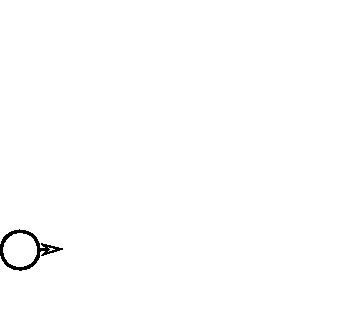
\includegraphics[width=0.44\textwidth]{slam_example_gt1.pdf}}
        }\hfill{}
        \subfloat[Sistema de SLAM del robot]
        {
            \fbox{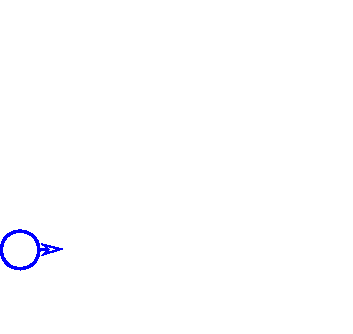
\includegraphics[width=0.44\textwidth]{slam_example_robot1.pdf}}
        }
    \end{figure}
    
\end{frame}

\begin{frame}
    \frametitle{Ejemplo de SLAM}
    
    \begin{figure}
        \subfloat[Realidad]
        {
            \fbox{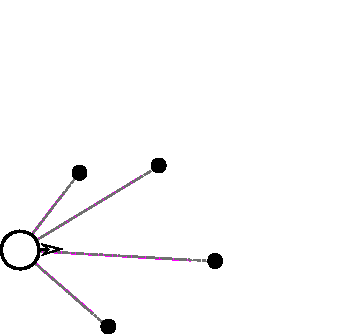
\includegraphics[width=0.44\textwidth]{slam_example_gt2.pdf}}
        }\hfill{}
        \subfloat[Sistema de SLAM del robot]
        {
            \fbox{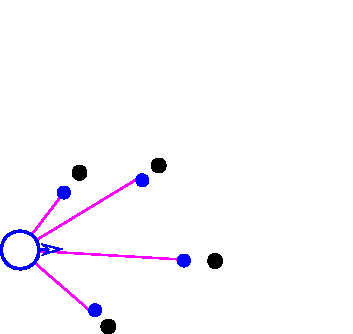
\includegraphics[width=0.44\textwidth]{slam_example_robot2.pdf}}
        }
    \end{figure}
    
\end{frame}

\begin{frame}
    \frametitle{Ejemplo de SLAM}
    
    \begin{figure}
        \subfloat[Realidad]
        {
            \fbox{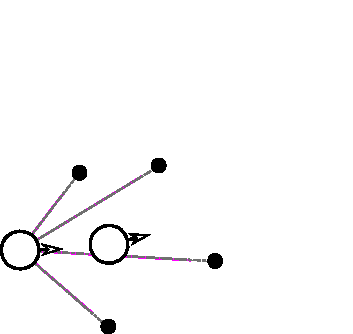
\includegraphics[width=0.44\textwidth]{slam_example_gt3.pdf}}
        }\hfill{}
        \subfloat[Sistema de SLAM del robot]
        {
            \fbox{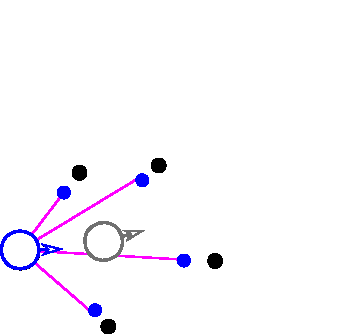
\includegraphics[width=0.44\textwidth]{slam_example_robot3.pdf}}
        }
    \end{figure}
    
\end{frame}

\begin{frame}
    \frametitle{Ejemplo de SLAM}
    
    \begin{figure}
        \subfloat[Realidad]
        {
            \fbox{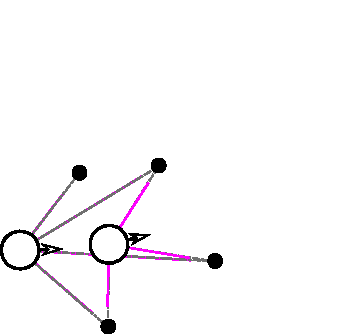
\includegraphics[width=0.44\textwidth]{slam_example_gt4.pdf}}
        }\hfill{}
        \subfloat[Sistema de SLAM del robot]
        {
            \fbox{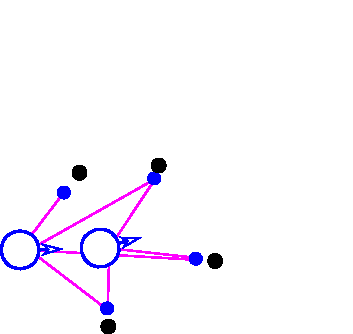
\includegraphics[width=0.44\textwidth]{slam_example_robot4.pdf}}
        }
    \end{figure}
    
\end{frame}

\begin{frame}
    \frametitle{Ejemplo de SLAM}
    
    \begin{figure}
        \subfloat[Realidad]
        {
            \fbox{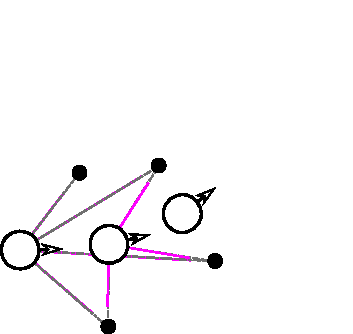
\includegraphics[width=0.44\textwidth]{slam_example_gt5.pdf}}
        }\hfill{}
        \subfloat[Sistema de SLAM del robot]
        {
            \fbox{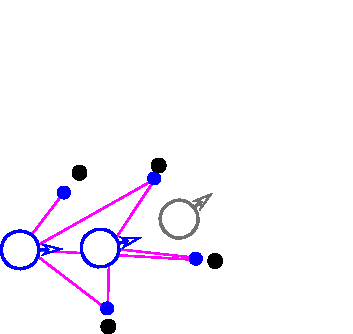
\includegraphics[width=0.44\textwidth]{slam_example_robot5.pdf}}
        }
    \end{figure}
    
\end{frame}

\begin{frame}
    \frametitle{Ejemplo de SLAM}
    
    \begin{figure}
        \subfloat[Realidad]
        {
            \fbox{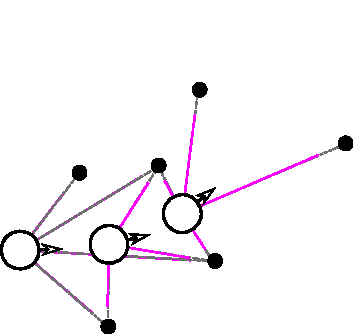
\includegraphics[width=0.44\textwidth]{slam_example_gt6.pdf}}
        }\hfill{}
        \subfloat[Sistema de SLAM del robot]
        {
            \fbox{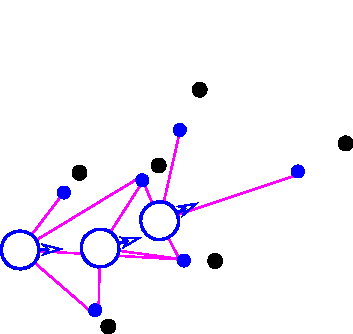
\includegraphics[width=0.44\textwidth]{slam_example_robot6.pdf}}
        }
    \end{figure}
    
\end{frame}

\begin{frame}
    \frametitle{Ejemplo de SLAM}
    
    \begin{figure}
        \subfloat[Realidad]
        {
            \fbox{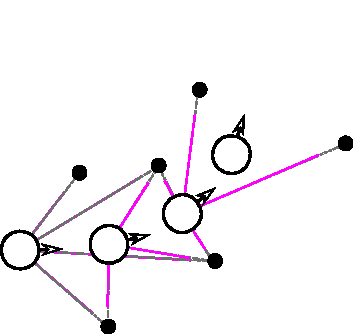
\includegraphics[width=0.44\textwidth]{slam_example_gt7.pdf}}
        }\hfill{}
        \subfloat[Sistema de SLAM del robot]
        {
            \fbox{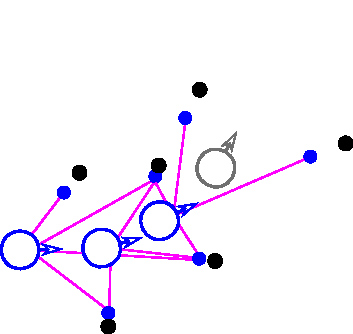
\includegraphics[width=0.44\textwidth]{slam_example_robot7.pdf}}
        }
    \end{figure}
    
\end{frame}

\begin{frame}
    \frametitle{Ejemplo de SLAM}
    
    \begin{figure}
        \subfloat[Realidad]
        {
            \fbox{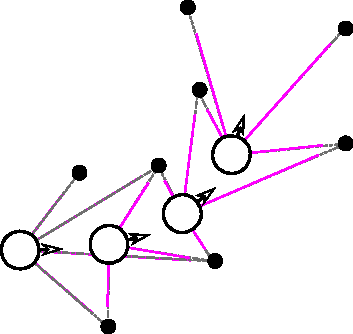
\includegraphics[width=0.44\textwidth]{slam_example_gt8.pdf}}
        }\hfill{}
        \subfloat[Sistema de SLAM del robot]
        {
            \fbox{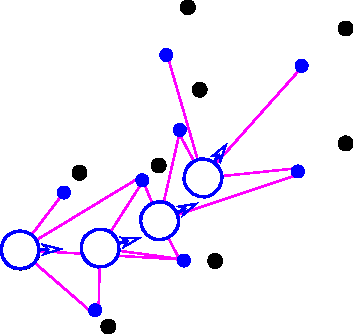
\includegraphics[width=0.44\textwidth]{slam_example_robot8.pdf}}
        }
    \end{figure}
    
\end{frame}

\begin{frame}
	\frametitle{Aquitectura general de SLAM}
	
	\begin{figure}[!h]
			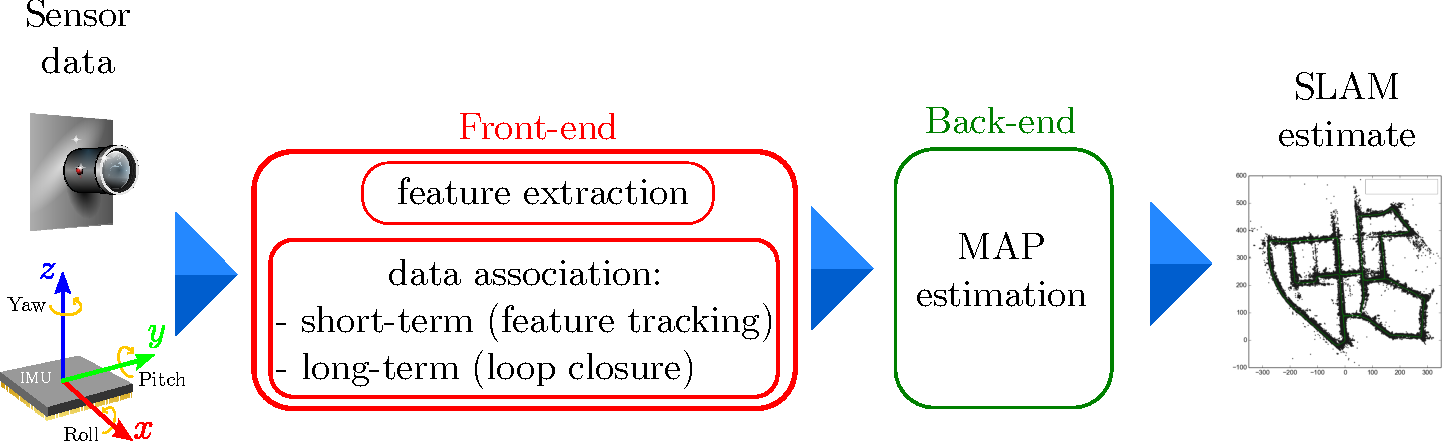
\includegraphics[width=\textwidth]{images/slam_frontend_backend.pdf}
	\end{figure}
	
\end{frame}

\begin{frame}
    \frametitle{Tipos de SLAM Back-ends}
    \note{Información extraída de https://youtu.be/BuRCJ2fegcc y de https://youtu.be/Alu59K8zvYs}
    \begin{itemize}
        \item Basados en Kalman Filter (EKF-SLAM)
        \item Basados en Particle Filter (FastSLAM, Rao-Blackwellized Particle Filter, Gmapping)
        \item Basados en Least-Squares (Graph-SLAM, Bundle Adjustment)
        \begin{itemize}
            \item Pose-Graph (solo contiene las poses del robot, el mapa es marginalizado\footnote{Marginalizar es el proceso de remover variables sin perder información.})
            \item Factor-Graph (contiene poses y landmarks)
        \end{itemize}
            Herramientas de optimización
            \begin{itemize}
            \item Ceres
            \item GTSAM
            \item g2o
            \end{itemize}
    \end{itemize}

	\begin{figure}[!h]
        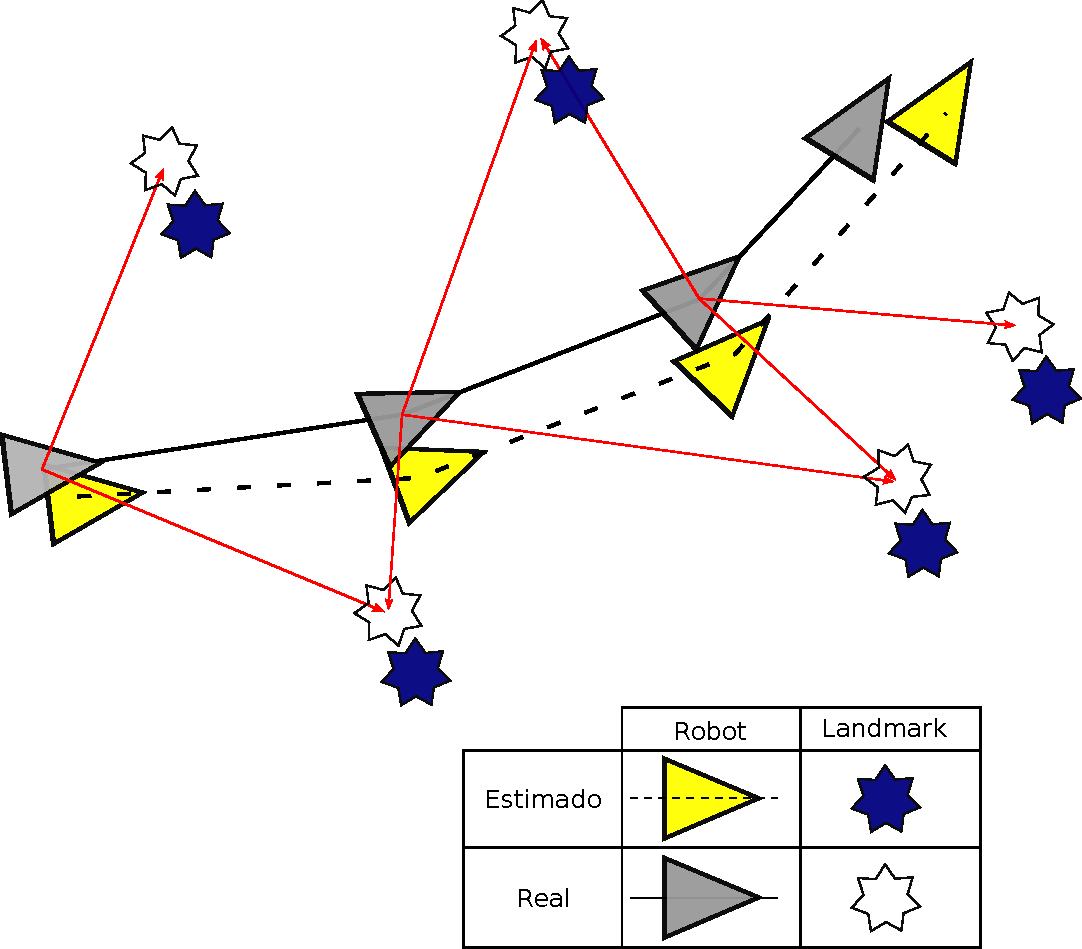
\includegraphics[width=0.2\textwidth]{images/slam-landmarks.pdf}
    \end{figure}
    
\end{frame}

\begin{frame}
    \frametitle{Graph-SLAM}
    
    Graph-SLAM: construir un grafo y encontrar una configuración de nodos que minimiza el error introducido por las restricciones (aristas)
    
    \begin{itemize}
        \item Se utiliza un grafo para representar el problema.
        \item Los nodos representan poses o ubicaciones de landmarks.
        \item Las aristas son observaciones de landmarks o mediciones de odometría
        \item La minimización optimiza las poses del robot y la ubicación del los landmarks
        \item Observar áreas previamente vistas genera restricciones en el grafo
    \end{itemize}

    \begin{figure}
    \subfloat[]
    {
        \fbox{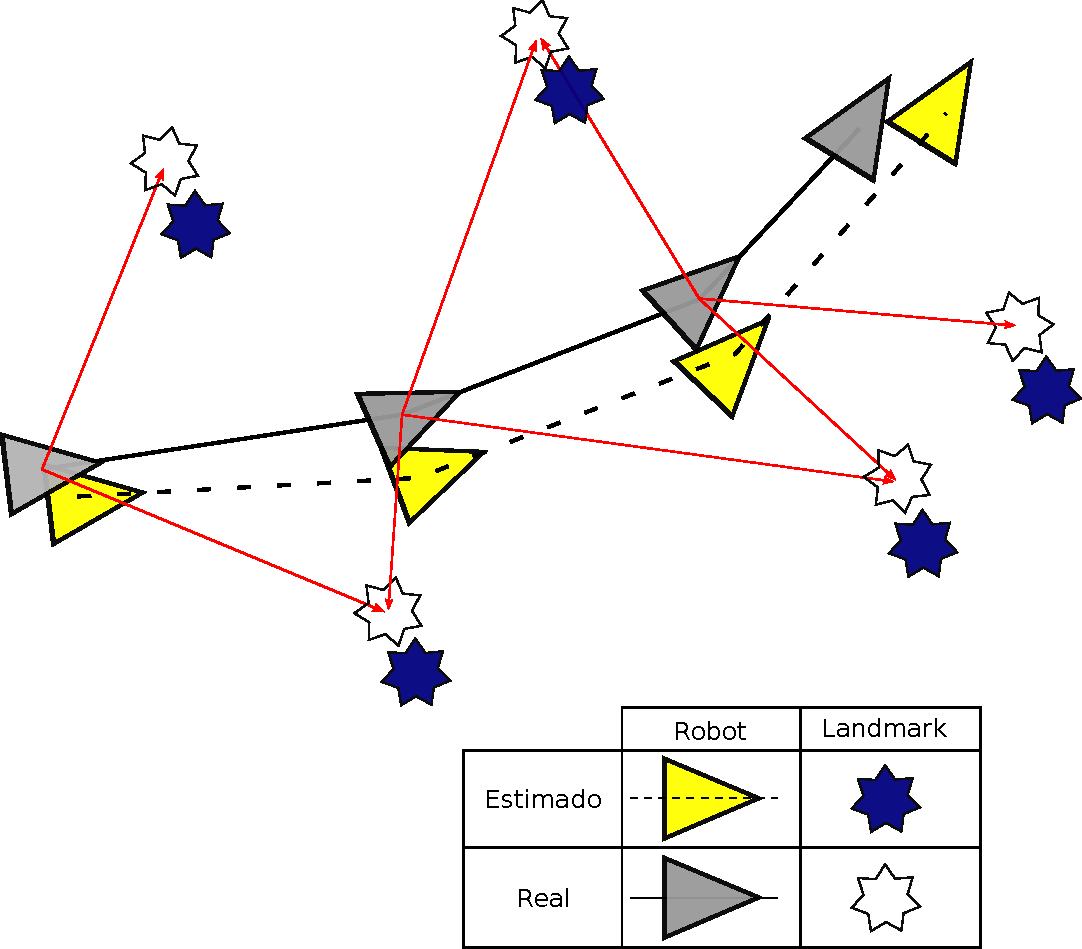
\includegraphics[width=0.25\textwidth]{images/slam-landmarks.pdf}}
    }\hspace{1em}
    \subfloat[]
    {
        \fbox{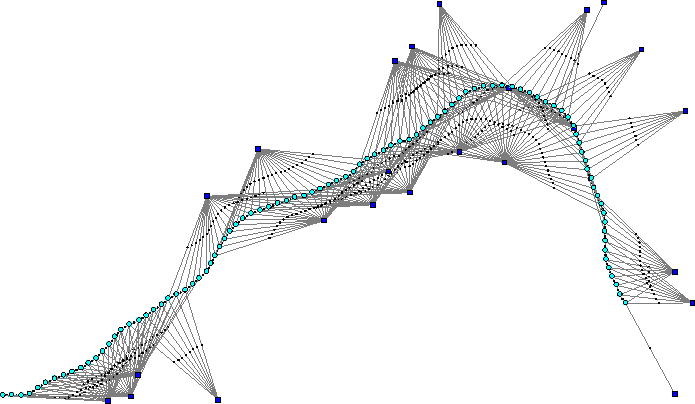
\includegraphics[width=0.375\textwidth]{images/factor_graph.pdf}}
    }
    \end{figure}
    
\end{frame}


\begin{frame}
    \frametitle{Factor-Graph}
    \note{Información extraída de https://youtu.be/uuiaqGLFYa4}
    
    \begin{block}{Factor-Graph}
        Un Factor-graph es un término matemático, un grafo bipartito representando la factorización de una función. Esto significa que podemos tomar una función por ejemplo $g(.)$ y descomponerla mediante el producto de funciones $f(.)$,
        
        \begin{equation*}
            g(X_{1}, \dots, X_{n}) = \prod_{i} f_{i}(S_{i}) \quad \text{con} \quad S_{i} 	\subseteq \{ X_{1},\dots, X_{n} \}
        \end{equation*}
    \end{block}

    \begin{figure}[!h]
        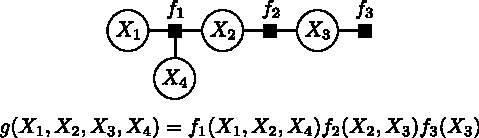
\includegraphics[width=0.7\textwidth]{images/factor_graph_example.pdf}
    \end{figure}

    \note{Por ejemplo, si la función g depende de 10 variables podemos descomponerla en el profucto de varias funciones f, donde cada función f depende de un subconjunto de esas variables.}
    
\end{frame}


\begin{frame}
    \frametitle{Factor-Graph}
    \note{Información extraída de https://youtu.be/uuiaqGLFYa4}
    
    \begin{itemize}
        \item Los Factor-Graph nos permiten representar una distribución de probabilidad conjunta (distribución que gobierna sobre todas las variables) como un producto de probabilidades más chicas (que dependen de un menor número de variables).
        \item Al igual que las redes de Bayes o redes de Markov, podemos utilizar los Factor-Graph para describir cómo las variables dependen entre si. Y podemos correr diferentes algoritmos sobre estos Factor-Graph para inferir información de una manera eficiente.
        \item Ejemplo de algorimo que trabaja sobre Factor-graph, es el Algoritmo de Sum-product para el computo de distribuciones marginales (distribuciones que solamente dependen un subconjunto de variables).
        \item En el contexto de robótica los Factor-graph son utilizados para especificar problemas de mínimos cuadrados. El factor graph nos permite representar cómo ciertos estados dependen o estan relacionados entre sí basados en la información que tenemos de las mediciones de los sensores (almacenada en los factores).
    \end{itemize}
    
    \note{Por ejemplo, si la función g depende de 10 variables podemos descomponerla en el profucto de varias funciones f, donde cada función f depende de un subconjunto de esas variables.}
    
\end{frame}

\begin{frame}
    \frametitle{Graph-based SLAM usando Pose-Graph}
    \note{Información extraída de https://youtu.be/uHbRKvD8TWg}
    
    \begin{itemize}
		\item Las restricciones conectan las poses del robot mientras se desplaza
		\item Las restricciones tiene ruido
    \end{itemize}

	\begin{figure}[!h]
		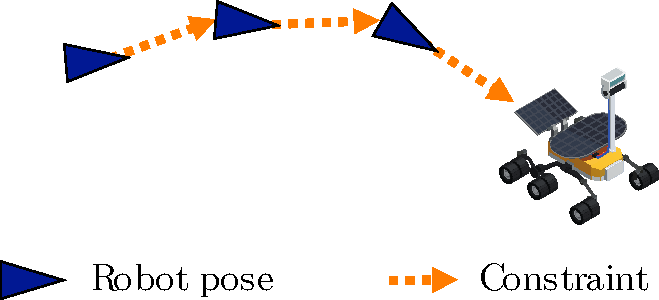
\includegraphics[width=0.7\textwidth]{images/pose_graph_example.pdf}
	\end{figure}
    
\end{frame}

\begin{frame}
    \frametitle{Graph-based SLAM usando Pose-Graph}
    \note{Información extraída de https://youtu.be/uHbRKvD8TWg}
    
    \begin{itemize}
    	\item Observando áreas previamente vistas se generan restricciones entre poses no consecutivas (\emph{Loop Closure})
    \end{itemize}
    
   	\begin{figure}[!h]
    	\includegraphics[width=0.4\textwidth]{images/pose_graph_loop_example.pdf}
    \end{figure}
    
\end{frame}

\begin{frame}[fragile]
    \frametitle{2D Pose-Graph con LiDAR}
    \note{Víðeo extraído de https://youtu.be/E6IvbjZA7Ao}
        
	\begin{center}
    \movie[loop]{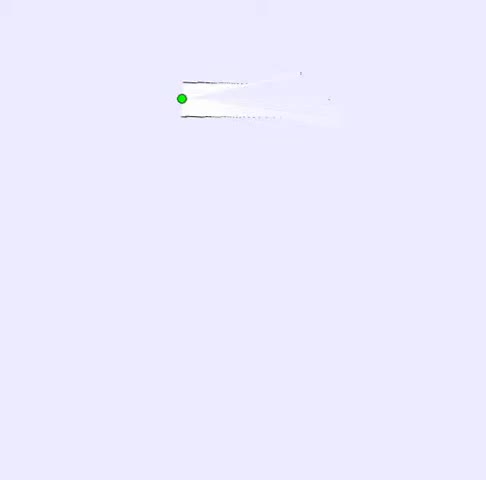
\includegraphics[width=0.5\columnwidth]{./images/pose_graph_2d_video.jpg}}{./videos/pose_graph_2d.mp4}
    \end{center}
    
\end{frame}


\begin{frame}
    \frametitle{Graph-based SLAM usando Pose-Graph}
    \note{Información extraída de https://youtu.be/uHbRKvD8TWg}
    
    \begin{columns}
        \begin{column}{0.5\textwidth}
        \begin{itemize}
            \item<1-2> Cada nodo es una pose del robot junto con su medición de laser (no hay landmarks)
            \item<1-2> Cada arista corresponde a una restricción espacial entre los nodos que relaciona.
            \item<3-> Una vez que tenemos el grafo, obtenemos el mapa mas probable mediante la corrección de los nodos
            \item<4-> así...
            \item<5> Dibujamos el mapa basandonos en las poses corregidas
        \end{itemize}
        \end{column}
        \begin{column}{0.5\textwidth}  %%<--- here
                \only<1>{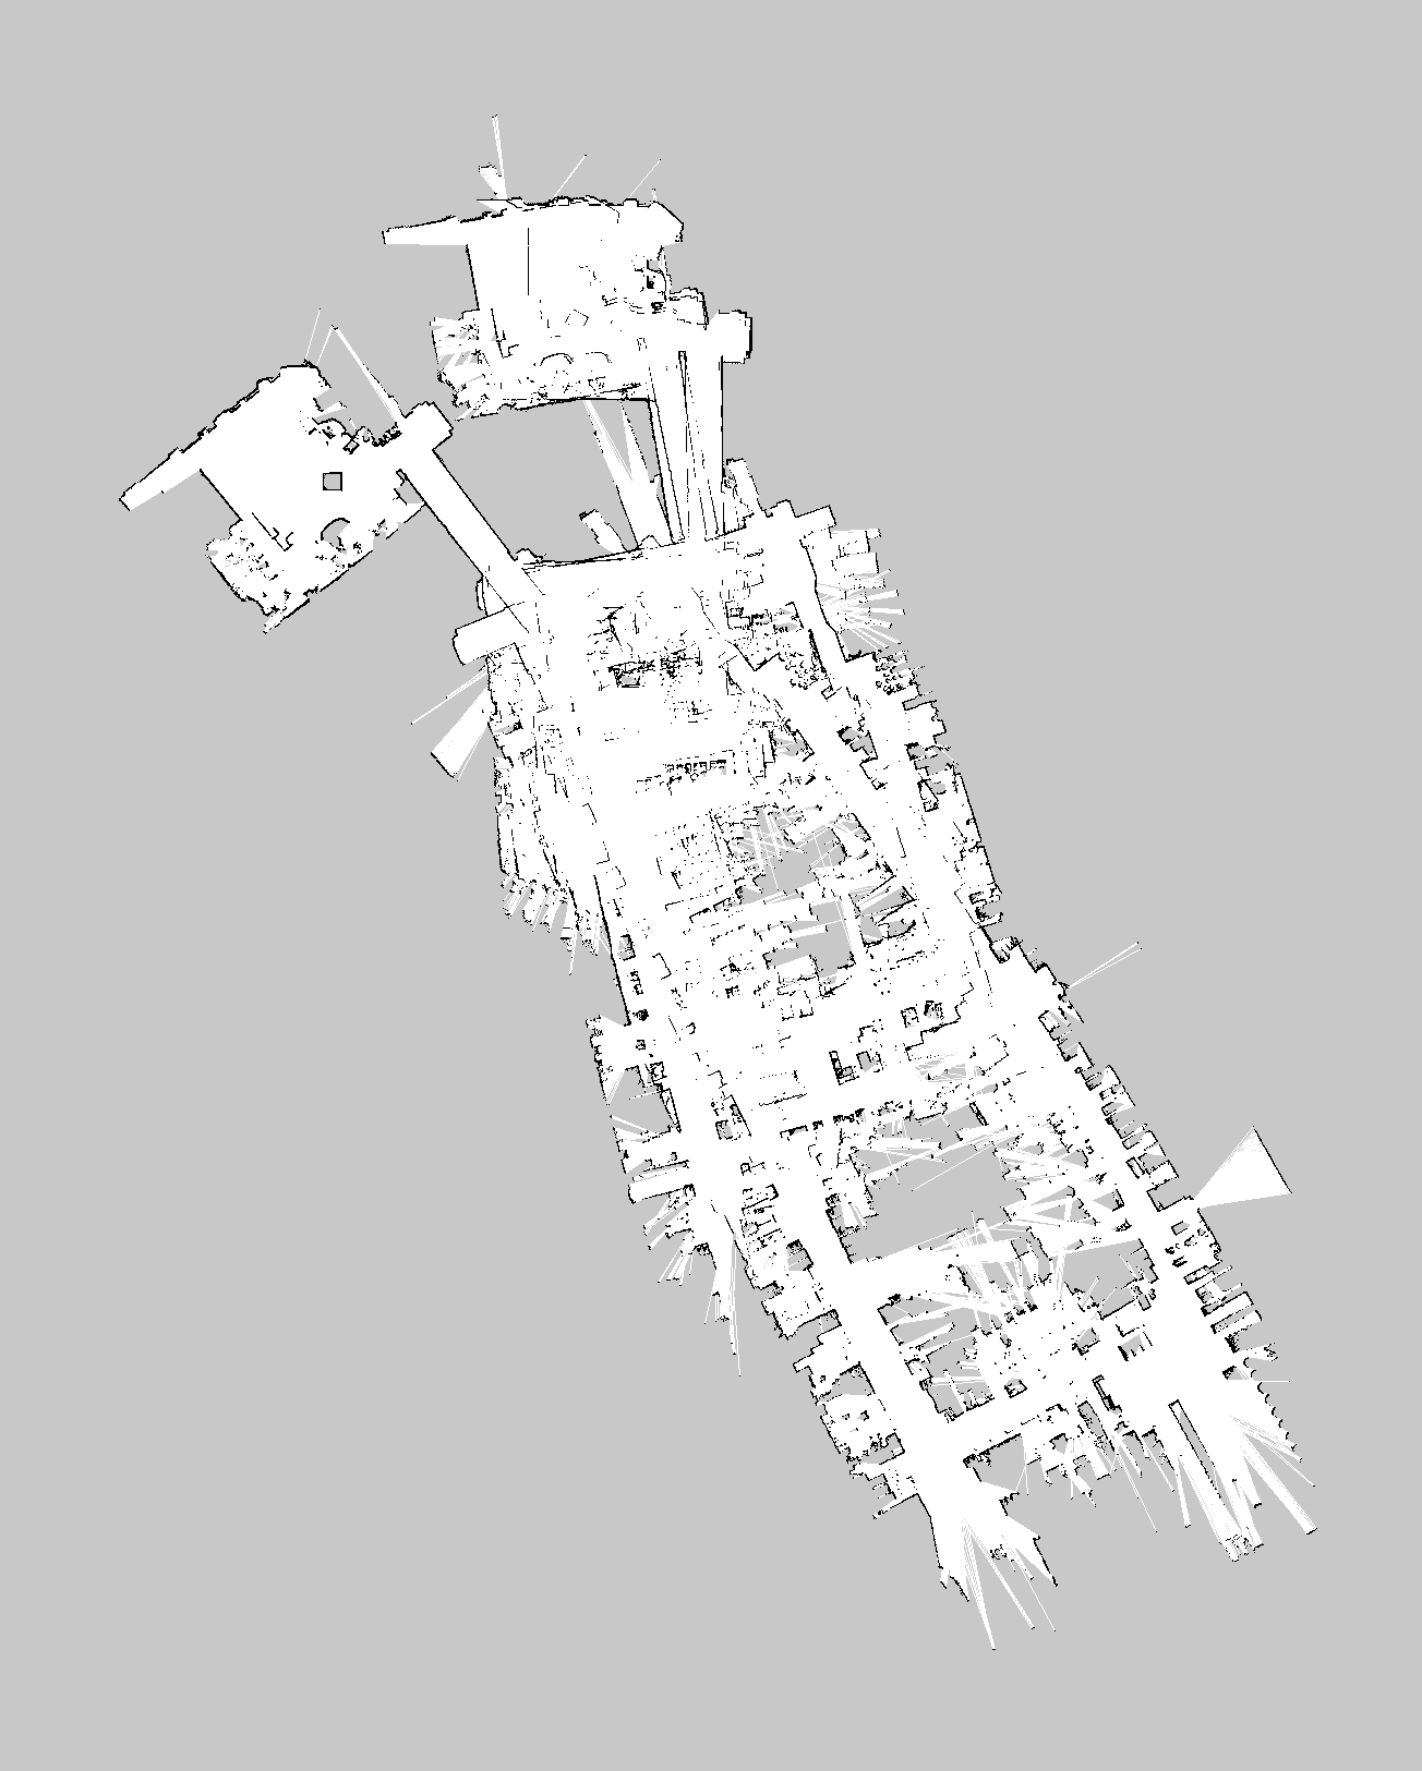
\includegraphics[width=0.7\textwidth]{images/pose_graph_map.png}}
                \only<2>{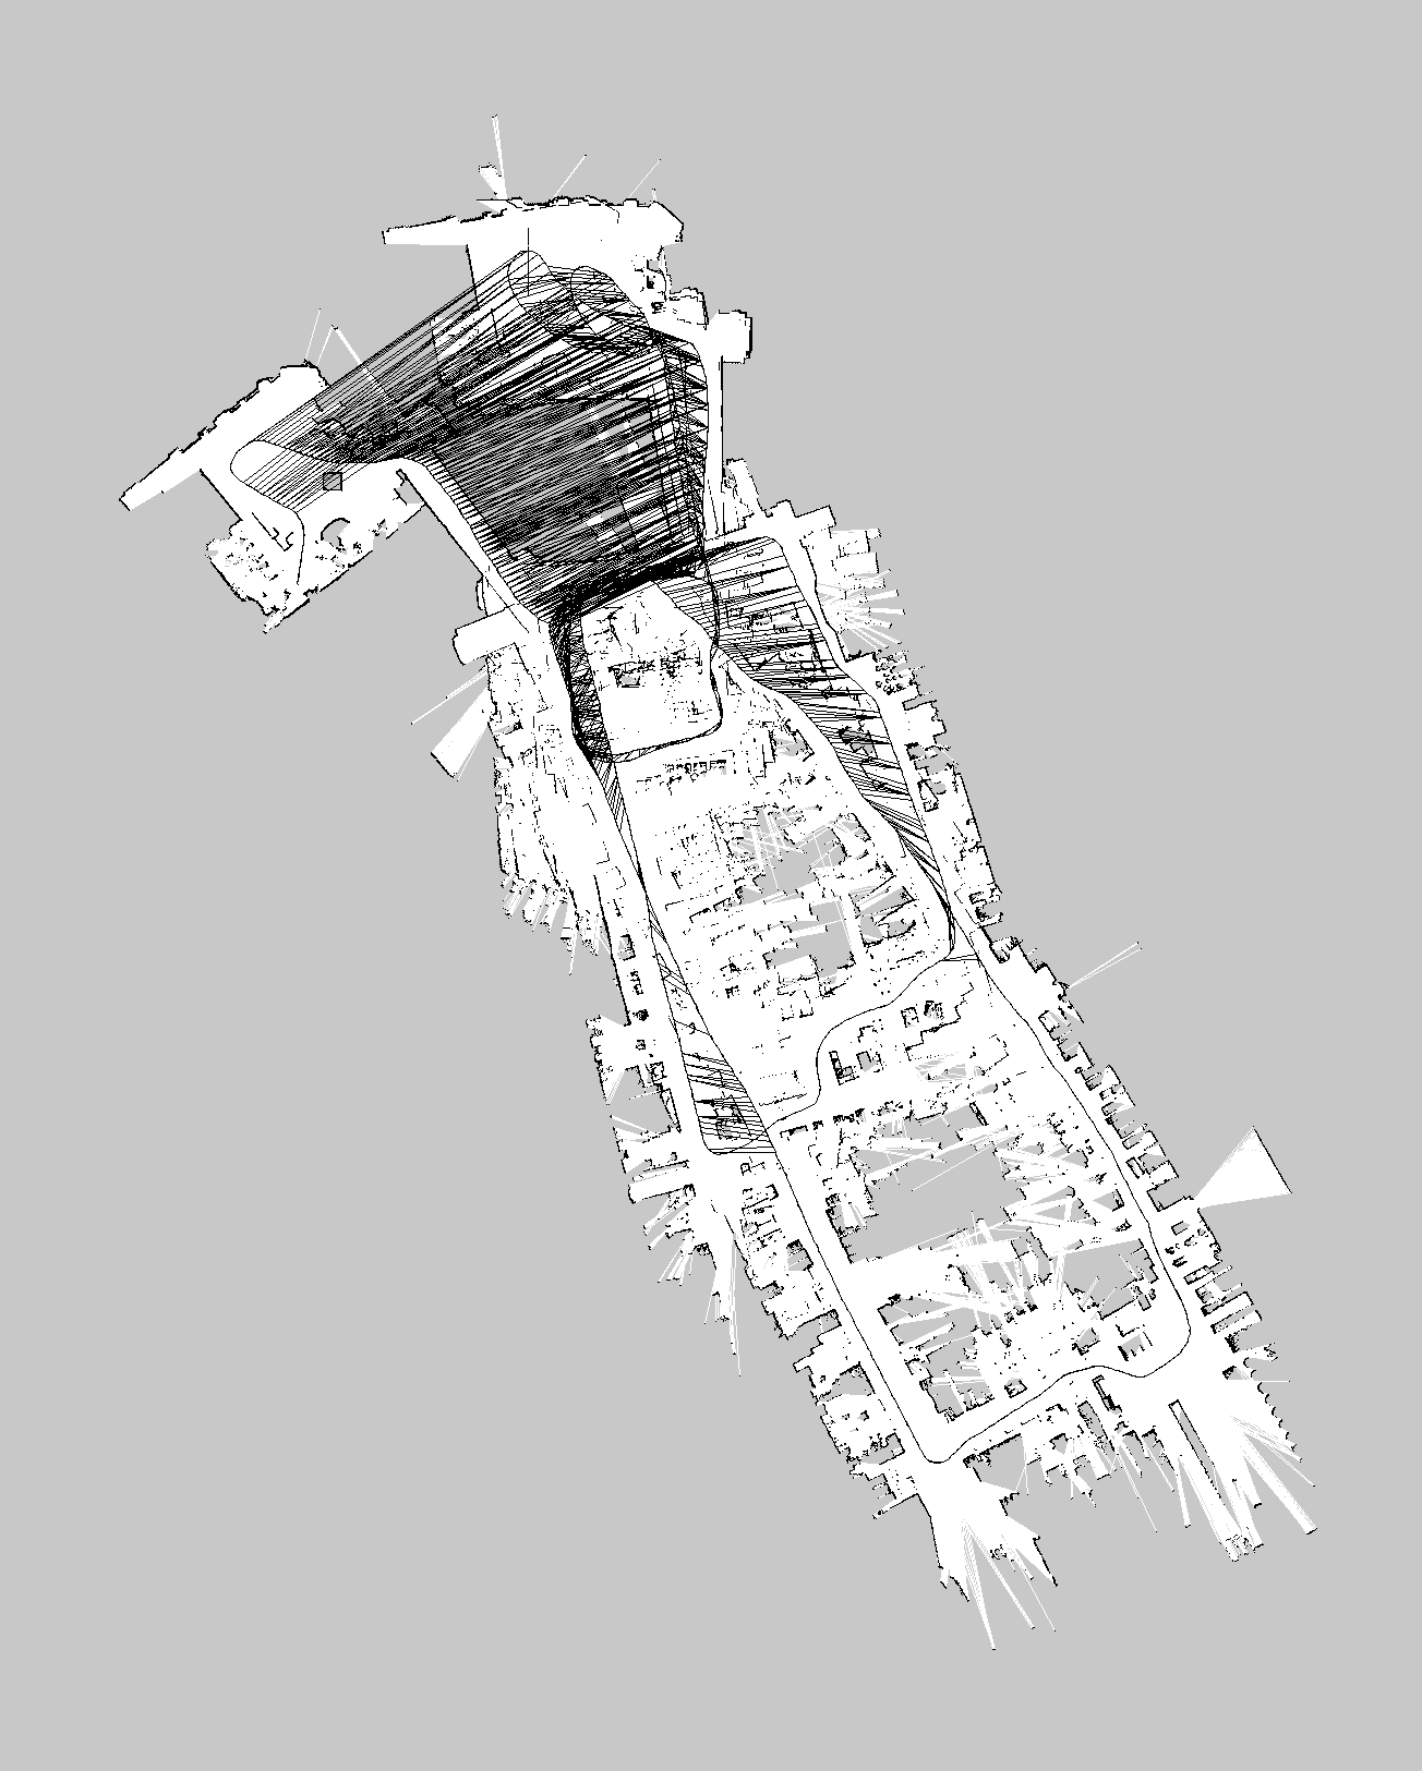
\includegraphics[width=0.7\textwidth]{images/pose_graph_constraints_with_map.png}}
                \only<3>{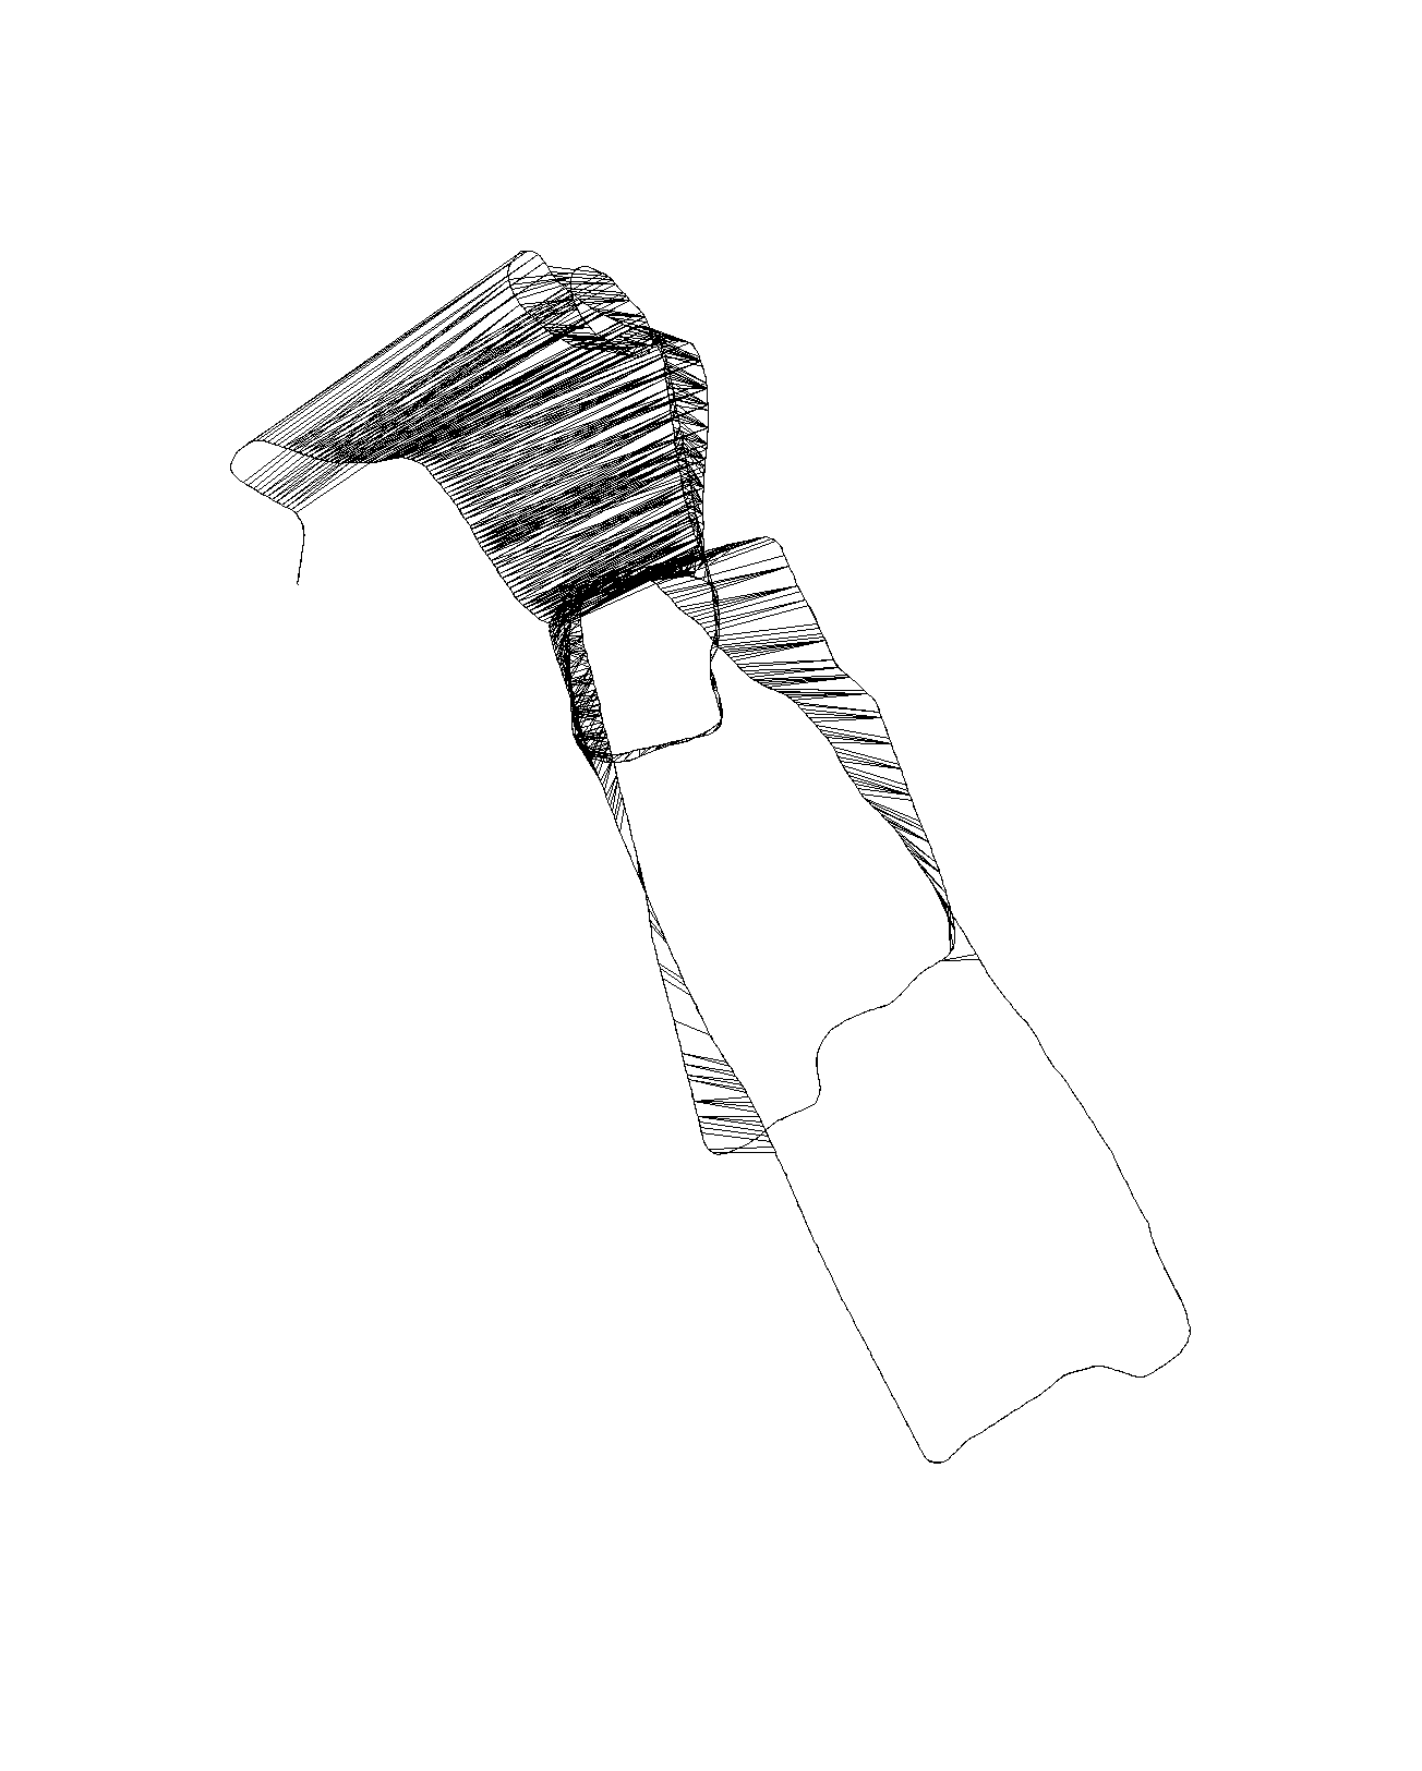
\includegraphics[width=0.7\textwidth]{images/pose_graph_constraints.png}}
                \only<4>{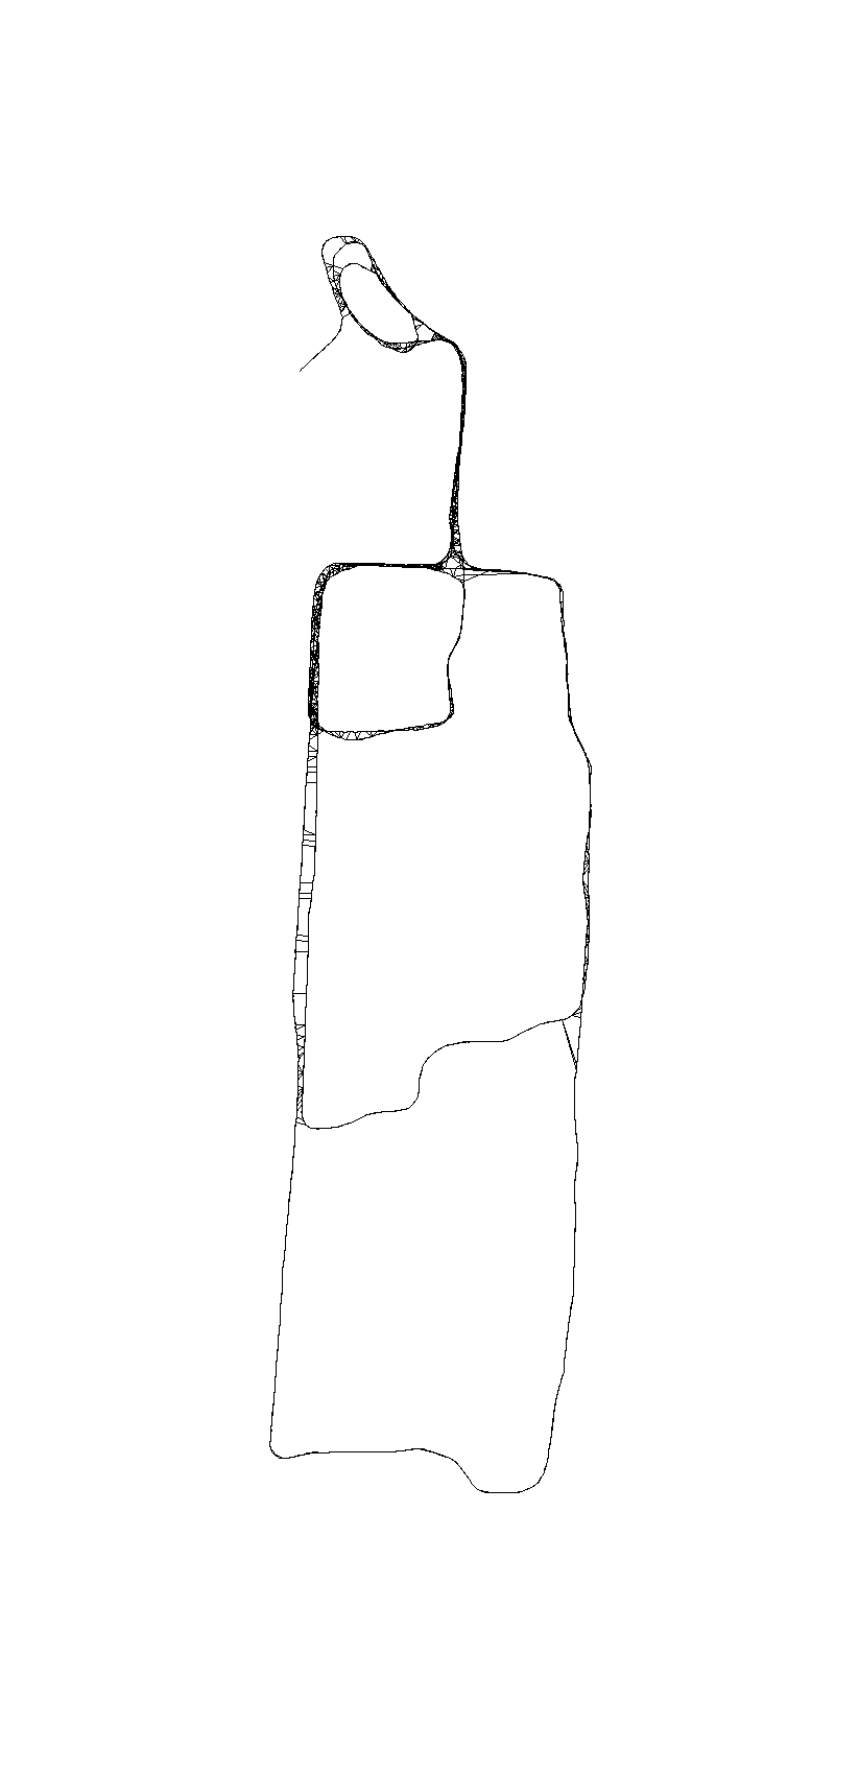
\includegraphics[width=0.5\textwidth]{images/pose_graph_optimized.png}}
                \only<5>{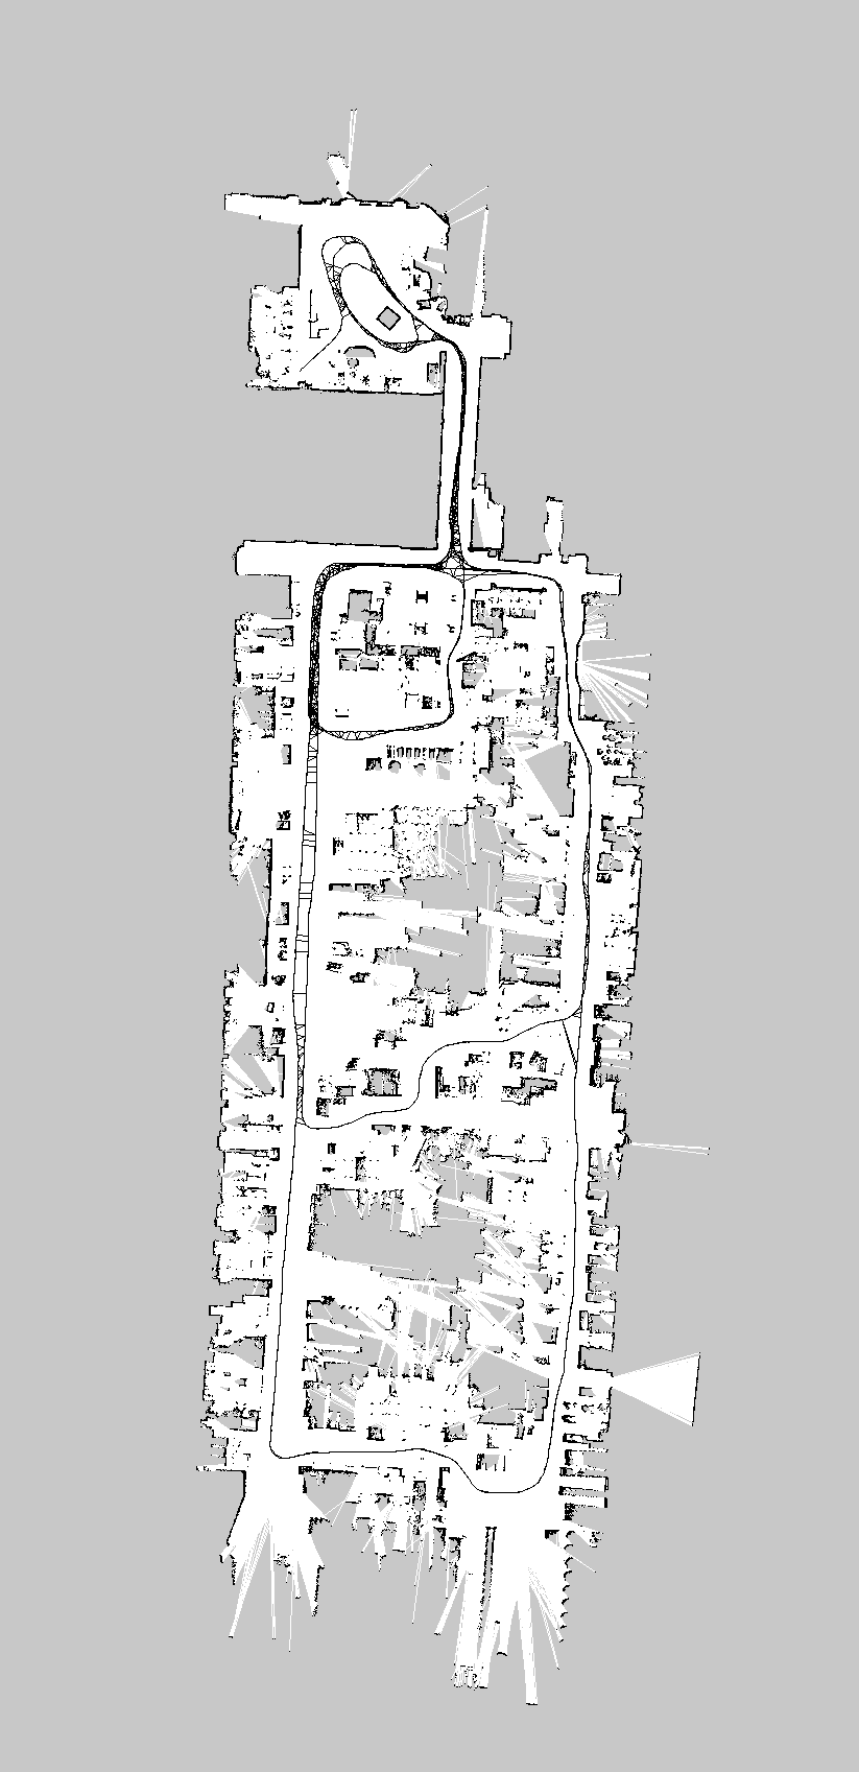
\includegraphics[width=0.5\textwidth]{images/pose_graph_optimized_with_map.png}}
        \end{column}
    \end{columns}
    
\end{frame}

\begin{frame}
	\frametitle{El grafo en pose-graph}
	\note{Información extraída de https://youtu.be/uHbRKvD8TWg}
	
	\begin{itemize}
		\item Consiste en $n$ nodos $\stateBold = \stateBold_{1:n}$
		\item Cada $\stateBold_{i}$ es una pose del robot en el tiempo $t_{i}$
		\item Una restricción/arista existe entre el nodo $\stateBold_{i}$ y $\stateBold_{j}$ si ...
	\end{itemize}
	
 	\begin{figure}[!h]
		\includegraphics[width=0.3\textwidth]{pose_graph_loop_example.pdf}
	\end{figure}
	
\end{frame}

\begin{frame}
	\frametitle{Crear una arista si...}
	\note{Información extraída de https://youtu.be/uHbRKvD8TWg}
	
	\begin{itemize}
		\item Una restricción/arista existe entre el nodo $\stateBold_{i}$ y $\stateBold_{j}$ si el robot se mueve de $\stateBold_{i}$ a $\stateBold_{i+1}$
		\item Las aristas corresponden a odometría
	\end{itemize}
	
	\begin{figure}[!h]
		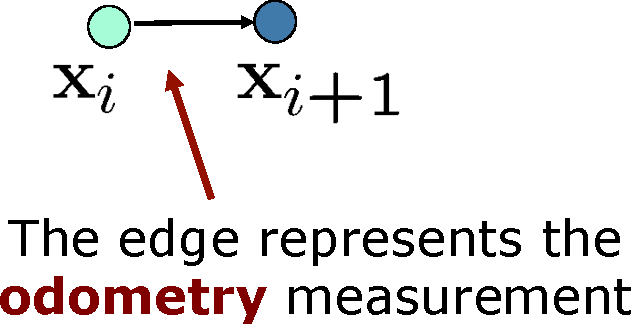
\includegraphics[width=0.44\textwidth]{pose_graph_odometry_edge.pdf}
	\end{figure}
	
\end{frame}


\begin{frame}
	\frametitle{Crear una arista si...}
	\note{Información extraída de https://youtu.be/uHbRKvD8TWg}
	
	\begin{itemize}
		\item<1-> Una restricción/arista existe entre el nodo $\stateBold_{i}$ y $\stateBold_{j}$ si el robot observa la misma parte del entorno desde $\stateBold_{i}$ y desde $\stateBold_{j}$
		\item<2>  Construimos una {\bf restricción virtual} entre la posición de $\stateBold_{j}$ vista desde $\stateBold_{i}$
	\end{itemize}
	\only<1>{
		\begin{figure}
			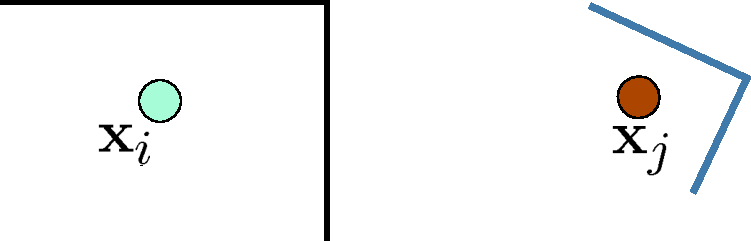
\includegraphics[width=0.44\textwidth]{pose_graph_edge_lidar.pdf}
		\end{figure}
	}
	\only<2>{
		\begin{figure}
			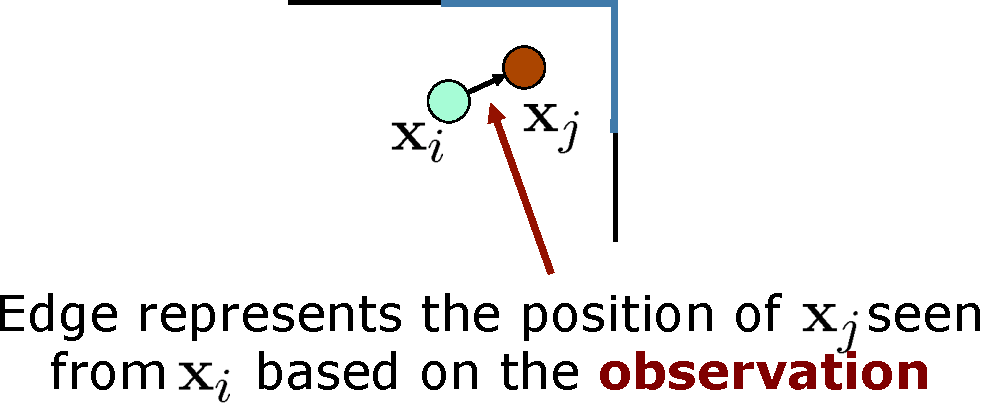
\includegraphics[width=0.44\textwidth]{pose_graph_edge_lidar2.pdf}
		\end{figure}
	}
	
\end{frame}

\begin{frame}
	\frametitle{La matriz de información de las aristas}
	\note{Información extraída de https://youtu.be/uHbRKvD8TWg}
    \begin{itemize}
		\item Las observaciones tienen ruido
		\item La matriz de información $\informationMatrix_{ij}$ para cada arista codifica su incertidumbre
		\item Mientras más grande $\informationMatrix_{ij}$, más importa la arista en al optimización.
	\end{itemize}
	
\end{frame}

\begin{frame}
	\frametitle{La matriz de información de las aristas}
	\note{Información extraída de https://youtu.be/uHbRKvD8TWg}
    \begin{figure}[!h]
		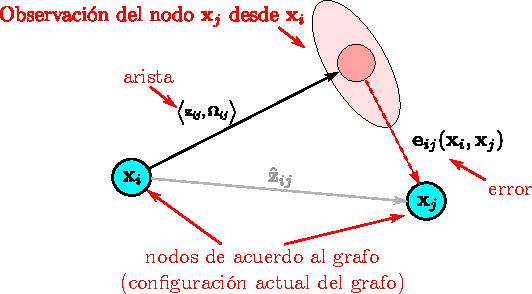
\includegraphics[width=0.7\textwidth]{images/factor_graph_edge_example.pdf}
	\end{figure}

	Objetivo:
	\begin{equation*}
		\stateBold^{*} = \argmin_{\stateBold} \sum_{ij} \error^{\top}_{ij} \informationMatrix_{ij} \error_{ij}
	\end{equation*}
	
\end{frame}



\begin{frame}
	\frametitle{Mínimos cuadrados en SLAM}
	\note{Información extraída de https://youtu.be/uHbRKvD8TWg}
	Podemos minimizar el error utilizaremos mínimos cuadrados (\emph{Least Square})
	\begin{align*}
		\state^{*} &= \argmin_{\stateBold} \sum_{ij} \error^{\top}_{ij}(\stateBold_{i},\stateBold_{j}) \informationMatrix_{ij} \error_{ij}(\stateBold_{i},\stateBold_{j})\\
	   		  &= \argmin_{\stateBold} \sum_{k} \error^{\top}_{k}(\stateBold) \informationMatrix_{k} \error_{k}(\stateBold)
	\end{align*}
	
	El {\bf vector estado} es la concatenación de los nodos pose $\stateBold = (\stateBold_{1}^{\top} \stateBold_{2}^{\top} \dots \stateBold_{n}^{\top})$. Cada nodo es una pose (posición u orientación).
	
    \vspace{2em}
	{\bf Tenemos que definir la función de error...}
\end{frame}


\begin{frame}
	\frametitle{Función de error}
	\note{Información extraída de https://youtu.be/uHbRKvD8TWg}
    
    \begin{itemize}
    \item Función de error para una sola restricción
       	\begin{figure}
            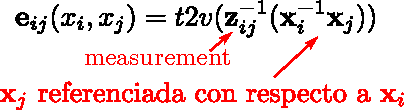
\includegraphics[width=0.44\textwidth]{pose_graph_error_function.pdf}
        \end{figure}
    \footnotetext{$t2v(.)$ mapea transformaciones a vectores}
    
    \item Error como una función de un vector estado completo
    
    \begin{equation*}
        \error_{ij}(\state) = t2v(\inverse{\observationBold}_{ij}(\inverse{\stateBold}_{i}\stateBold_{j}))
    \end{equation*}

    \item El error toma el valor 0 cuando
    
    \begin{equation*}
        \inverse{\observationBold}_{ij} = (\inverse{\stateBold}_{i}\stateBold_{j})
    \end{equation*}
    
    \end{itemize}
\end{frame}

\begin{frame}
	\frametitle{Método de Gauss-Newton para la minimización del error}
	\note{Información extraída de https://youtu.be/uHbRKvD8TWg}
    
    \TODO{especificar metamáticamente estos pasos, sino no se entiende porque hay que linearizar el error. Ni cómo llegamos a construir el sistema lineal ni por qué.}
    
    \begin{itemize}
        \item Definir la función de error
        \item Linearizar la función de error
        \item Calcular las derivadas
        \item Igualar las derivadas a cero
        \item Resolver el sistema lineal
        \item Iterar este procedimiento hasta que converja
    \end{itemize}
    
	
\end{frame}

\begin{frame}
	\frametitle{Linearizar la función de error}
	\note{Información extraída de https://youtu.be/uHbRKvD8TWg}
    
    \begin{itemize}
        \item Podemos aproximar el error al rededor de una estimación inicial $\state$ a través de una expansión de Taylor
    \end{itemize}

    \begin{equation*}
        \error_{ij}(\stateBold + \vec{\Delta}\stateBold) \simeq  \error_{ij}(\stateBold) + \jacobian_{ij}\vec{\Delta}\stateBold \quad \text{con} \quad \jacobian_{ij} = \dfrac{\partial\error_{ij}(\stateBold)}{\partial\stateBold}
    \end{equation*}
	
\end{frame}

\begin{frame}
	\frametitle{Derivada de la función de error}
	\note{Información extraída de https://youtu.be/uHbRKvD8TWg}
    \begin{itemize}
        \item<1-> Pregunta: ¿Depende un término de error $\error_{ij}(\stateBold)$ de todas las variables de estado?
        
        \only<2->{No, solo depende de $\stateBold_{i}$ y $\stateBold_{j}$}
        
        \item<3-> Pregunta: ¿Hay alguna consecuencia en la estructura del Jacobiano?
        
        \only<4->{
        	Si, será diferente a cero solamente en las filas correspondientes a  $\stateBold_{i}$ y $\stateBold_{j}$
        
	        \begin{align*}
	            \dfrac{\partial\error_{ij}(\stateBold)}{\partial\stateBold} &= 
	            \begin{bmatrix}
	                0 & \dots & \dfrac{\partial\error_{ij}(\stateBold_{i})}{\partial\stateBold_{i}} & \dots & 0 & \dots & \dfrac{\partial\error_{ij}(\stateBold_{j})}{\partial\stateBold_{j}} & \dots & 0
	            \end{bmatrix} \\
	            \jacobian_{ij} &= 
	                \begin{bmatrix}
	                    0 & \dots & \vec{A}_{ij} & \dots & 0 & \dots & \vec{B}_{ij} & \dots & 0
	                \end{bmatrix}
	        \end{align*}
	    }
        
        
    \end{itemize}
	
\end{frame}


\begin{frame}
	\frametitle{Jacobianos y problema disperso}
	\note{Información extraída de https://youtu.be/uHbRKvD8TWg}
	
	\begin{itemize}
		\item El error $\error_{ij}(\stateBold)$ depende solamente de los bloques de parámetros $\stateBold_{i}$ y $\stateBold_{j}$
		
		\begin{equation*}
			\error_{ij}(\stateBold) =\error_{ij}(\stateBold_{i} ,\stateBold_{j})
		\end{equation*}
	
		\item El Jacobiano será cero en todos lados excepto en las columnas $\stateBold_{i}$ y $\stateBold_{j}$
		
   		\begin{equation*}
			\jacobian_{ij} = 
			\begin{bmatrix}
				0 & \dots & 0 & \dfrac{\partial\error_{ij}(\stateBold_{i})}{\partial\stateBold_{i}} & 0 & \dots & 0 & \dfrac{\partial\error_{ij}(\stateBold_{j})}{\partial\stateBold_{j}} & 0 & \dots & 0
			\end{bmatrix}
		\end{equation*}
		
	\end{itemize}

	{\bf Esto nos permite resolver SLAM de manera eficiente!}
	
\end{frame}


\begin{frame}
	\frametitle{Consecuencia de que sea un problema disperso}
	\note{Información extraída de https://youtu.be/uHbRKvD8TWg}
	
	\begin{itemize}
		\item Necesitamos computar el vector coeficiente
		\begin{align*}
			\linearSystemb^{\top} &= \sum_{ij} \linearSystemb_{ij}^{\top} = \sum_{ij} \error_{ij}^{\top}\Omega_{ij}\jacobian_{ij}\\
			\linearSystemH &= \sum_{ij} \linearSystemH_{ij} = \sum_{ij} \jacobian_{ij}^{\top}\Omega_{ij}\jacobian_{ij}
		\end{align*}
		\item La estructura dispersa de $\jacobian_{ij}$ resultará en una estructura dispersa de $\linearSystemH$
		\item Esta estructura refleja la matriz de adyacencia del grafo
	\end{itemize}
	
\end{frame}

\begin{frame}
	\frametitle{Ilustración de la estructura}
	\note{Información extraída de https://youtu.be/uHbRKvD8TWg}
	
    \begin{figure}[!h]
		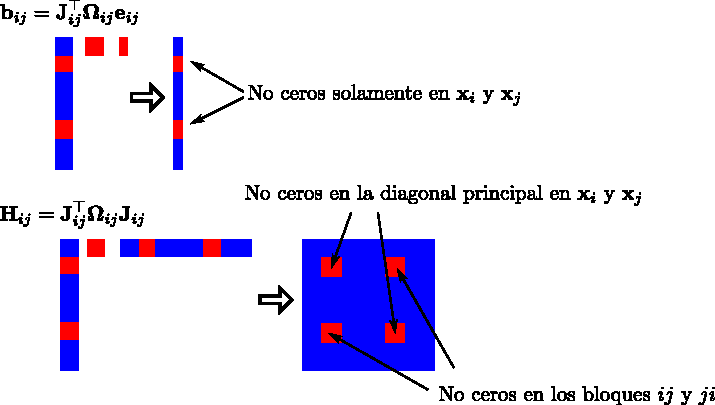
\includegraphics[width=0.9\textwidth]{linear_system_sparsity.pdf}
	\end{figure}
	
\end{frame}

\begin{frame}
	\frametitle{Consecuencia de que sea un problema disperso}
	\note{Información extraída de https://youtu.be/uHbRKvD8TWg}
	
 	\begin{figure}[!h]
		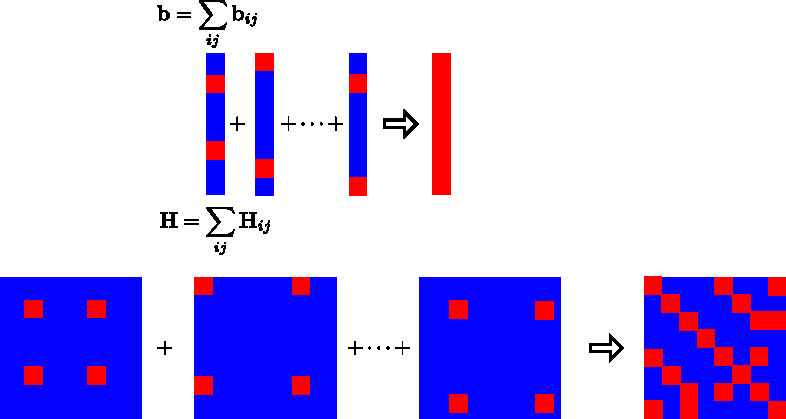
\includegraphics[width=0.9\textwidth]{linear_system_sparsity2.pdf}
	\end{figure}
	
\end{frame}

\begin{frame}
	\frametitle{Consecuencia de que sea un problema disperso}
	\note{Información extraída de https://youtu.be/uHbRKvD8TWg}
	
	\begin{itemize}
		\item Una arista contribuye al sistema lineal a través de $\linearSystemb_{ij}$ y $\linearSystemH_{ij}$
		\item El vector coeficiente es
		
		\begin{align*}
			\linearSystemb_{ij}^{\top} &= \error_{ij}^{\top}\informationMatrix_{ij}\jacobian_{ij}\\
			&= \error_{ij}^{\top}\informationMatrix_{ij}
				\begin{bmatrix}
					0 & \dots & \vec{A}_{ij} & \dots & \vec{B}_{ij} & \dots & 0
				\end{bmatrix}\\
			&= 
				\begin{bmatrix}
					0 & \dots & \error_{ij}^{\top}\informationMatrix_{ij}\vec{A}_{ij} & \dots & \error_{ij}^{\top}\informationMatrix_{ij}\vec{B}_{ij} & \dots & 0
				\end{bmatrix}
		\end{align*}
		\item Es diferente a cero solamente en los índices correspondientes de $\stateBold_{i}$ y $\stateBold_{j}$		
	\end{itemize}
	
\end{frame}

\begin{frame}
	\frametitle{Consecuencia de que sea un problema disperso}
	\note{Información extraída de https://youtu.be/uHbRKvD8TWg}
	
	\begin{itemize}
		\item La matriz coeficiente de una arista es

		\begin{align*}
			\linearSystemH_{ij}^{\top} &= \jacobian_{ij}^{\top}\informationMatrix_{ij}\jacobian_{ij}\\
			&= 
			\begin{bmatrix}
				\vdots \\
				\vec{A}_{ij}^{\top}\\
				\vdots \\
				\vec{B}_{ij}^{\top}\\
				\vdots
			\end{bmatrix} \informationMatrix_{ij}
			\begin{bmatrix}
				\cdots & \vec{A}_{ij} & \cdots & \vec{B}_{ij} & \cdots
			\end{bmatrix}\\
			&= 
			\begin{bmatrix}
				\vec{A}_{ij}^{\top}\informationMatrix_{ij}\vec{A}_{ij} & \vec{A}_{ij}^{\top}\informationMatrix_{ij}\vec{B}_{ij}\\
				\vec{B}_{ij}^{\top}\informationMatrix_{ij}\vec{A}_{ij} & \vec{B}_{ij}^{\top}\informationMatrix_{ij}\vec{B}_{ij}
			\end{bmatrix}
		\end{align*}
		\item Es diferente a cero en los bloques relacionados con $i,j$
	\end{itemize}
	
\end{frame}


\begin{frame}
	\frametitle{Resumen del problema disperso}
	\note{Información extraída de https://youtu.be/uHbRKvD8TWg}
	
	\begin{itemize}
		\item Una arista ij solo contribuye a
		\begin{itemize}
			\item i-ésimo y j-ésimo bloques de $\linearSystemb_{ij}$
			\item los bloques $ii$, $jj$, $ij$ y $ji$ de $\linearSystemH_{ij}$
		\end{itemize}
		\item el sistema resultante es disperso
		\item El sistema se puede computar sumando las contribuciones de cada arista
		\item Se pueden utilizar diferentes solvers
		\begin{itemize}
			\item Descoposición de Sparse Cholesky
			\item Gradiente conjudado
			\item muchos más...
		\end{itemize}

	\end{itemize}
	
	
\end{frame}

\begin{frame}
	\frametitle{El sistema Lineal}
	\note{Información extraída de https://youtu.be/uHbRKvD8TWg}
	
	\begin{itemize}
		\item Vector de incrementos de estado
		\begin{equation*}
			\Delta\stateBold^{\top} =
			\begin{bmatrix}
			\Delta\stateBold_{1}^{\top}	& \Delta\stateBold_{2}^{\top} & \cdots & \Delta\stateBold_{n}^{\top}
			\end{bmatrix}
		\end{equation*}
	\item Vector coeficiente
		\begin{equation*}
			\linearSystemb^{\top} =
			\begin{bmatrix}
				\overline{\linearSystemb}_{1}^{\top} & \overline{\linearSystemb}_{2}^{\top} & \cdots & \overline{\linearSystemb}_{n}^{\top}
			\end{bmatrix}
		\end{equation*}
	\item Matriz de ecuaciones normales
		\begin{equation*}
			\linearSystemH =
			\begin{bmatrix}
			\overline{\linearSystemH}_{11} & \overline{\linearSystemH}_{12} & \cdots & \overline{\linearSystemH}_{1n}\\
			\overline{\linearSystemH}_{21} & \overline{\linearSystemH}_{22} & \cdots & \overline{\linearSystemH}_{2n}\\
			\vdots & \vdots & \ddots & \vdots\\
			\overline{\linearSystemH}_{n1} & \overline{\linearSystemH}_{n2} & \cdots & \overline{\linearSystemH}_{nn}\\
			\end{bmatrix}
		\end{equation*}
	\end{itemize}

\end{frame}

\begin{frame}
	\frametitle{Construcción del sistema lineal}
	\note{Información extraída de https://youtu.be/uHbRKvD8TWg}
	Para cada restricción:
	\begin{itemize}
		\item Computar el error $\error_{ij} = t2v(\inverse{\observationBold}_{ij}(\inverse{\stateBold}_{i}\stateBold_{j}))$
		\item Computar los bloques de los jacobianos:
			\begin{equation*}
				\vec{A}_{ij} = \dfrac{\partial\error_{ij}(\stateBold_{i}, \stateBold_{j})}{\partial\stateBold_{i}} \quad \quad \vec{B}_{ij} = \dfrac{\partial\error_{ij}(\stateBold_{i}, \stateBold_{j})}{\partial\stateBold_{j}}
			\end{equation*}
	\item Actualizar el vector coeficiente:
		\begin{equation*}
			\overline{\linearSystemb}_{i}^{\top} += \error_{ij}^{\top}\informationMatrix_{ij}\vec{A}_{ij} \quad \quad \overline{\linearSystemb}_{j}^{\top} += \error_{ij}^{\top}\informationMatrix_{ij}\vec{B}_{ij}
		\end{equation*}

	\item Actualizar el vector coeficiente:
		\begin{align*}
			\overline{\linearSystemH}_{ij}^{\top} &+= \vec{A}_{ij}^{\top}\informationMatrix_{ij}\vec{A}_{ij} \quad \quad \overline{\linearSystemH}_{ij}^{\top} += \vec{A}_{ij}^{\top}\informationMatrix_{ij}\vec{B}_{ij} \\
			\overline{\linearSystemH}_{ij}^{\top} &+= \vec{B}_{ij}^{\top}\informationMatrix_{ij}\vec{A}_{ij} \quad \quad \overline{\linearSystemH}_{ij}^{\top} += \vec{B}_{ij}^{\top}\informationMatrix_{ij}\vec{B}_{ij}
		\end{align*}
	\end{itemize}	
	
\end{frame}

\begin{frame}
	\frametitle{Algoritmo}
	\note{Información extraída de https://youtu.be/uHbRKvD8TWg}
	
	\begin{algorithmic}[1]
		\Procedure{optimize}{$\stateBold$}
		\While (!converged)
		\State $(\linearSystemH,\linearSystemb) = buildLinearSystem(\stateBold)$
		\State $\vec{\Delta}\stateBold = solveSparse(\linearSystemH\vec{\Delta}\stateBold = -\linearSystemb)$
		\State $\stateBold = \stateBold + \vec{\Delta}\stateBold$
		\EndWhile

		\State \Return $\stateBold$
		\EndProcedure
	\end{algorithmic}
	
\end{frame}


\begin{frame}
	\frametitle{Ejemplo Trivial 1D}
	\note{Información extraída de https://youtu.be/uHbRKvD8TWg}
	
    Dos nodos y una observación

 	\begin{figure}[!h]
        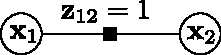
\includegraphics[width=0.2\textwidth]{pose_graph_1d_example.pdf}
    \end{figure}

    \small

    \begin{align*}
        \stateBold &=
        \begin{bmatrix}
            \stateBold_{1} & \stateBold_{2}
        \end{bmatrix}^{\top}
        =
        \begin{bmatrix}
            0 & 0
        \end{bmatrix}\\
        \observationBold_{12} &= 1\\
        \informationMatrix &= 2\\
        \error_{12} &= \observationBold_{12} - (\stateBold_{2} - \stateBold_{1}) = 1 - (0 - 0) = 1\\
	    \jacobian_{12} &=
	    \begin{bmatrix}
        	1 & -1
        \end{bmatrix}\\
        \linearSystemb_{12}^{\top} &= \error_{12}^{\top} \informationMatrix_{12} \jacobian_{12} =
        \begin{bmatrix}
            2 & -2
        \end{bmatrix}\\
        \linearSystemH_{12} &= \jacobian_{12}^{\top} \informationMatrix_{12} \jacobian_{12} = 
        \begin{bmatrix}
            2 & -2\\
            -2 & 2
        \end{bmatrix}\\
    \vec{\Delta}\stateBold &= -\inverse{\linearSystemH}_{12} \linearSystemb_{12}\\
    \end{align*}

    \begin{center}
    \alert{Problema:} $\det(\linearSystemH) = 0$, por lo tanto no podemos invertir $\linearSystemH$
    \end{center}
\end{frame}

\begin{frame}
	\frametitle{¿Qué es lo que anda mal?}
	\note{Información extraída de https://youtu.be/uHbRKvD8TWg}
    
    \begin{itemize}
        \item La restricción especifica una restricción relativa entre ambos nodos
        \item Cualquier pose de los nodos va a estar bien si se cumple la restricción relativa entre ellos. Este problema se lo conoce como {\bf Gauge Freedom}
        \item Para resolverlo tenemos que {\bf fijar} un nodo. Al fijar un nodo estamos agregando un {\bf Prior}!
    \end{itemize}

    \begin{align*}
        \linearSystemH &=
        \begin{bmatrix}
            2 & -2\\
            -2 & 2
        \end{bmatrix}
        +
        \begin{bmatrix}
            1 & 0\\
            0 & 0
        \end{bmatrix} \leftarrow \text{restricción que pone } \vec{\Delta}\stateBold_{1} = 0\\
        \vec{\Delta}\stateBold &= -\inverse{\linearSystemH}_{12} \linearSystemb_{12}\\
        \vec{\Delta}\stateBold &=
        \begin{bmatrix}
            0 & 1
        \end{bmatrix}^{\top}
    \end{align*}
    
    Con esto hacemos que el update del nodo $\stateBold_{1}$ sea 0 y que el update de $\stateBold_{2}$ sea actualizado con 1.
\end{frame}

\begin{frame}
    \frametitle{Rol del Prior}
    \note{Información extraída de https://youtu.be/uHbRKvD8TWg}
    
    \begin{itemize}
        \item Vimos que la matriz de información $\linearSystemH$ no es de rango completa, y por tanto no es invertible
        \item Un marco de referencia global no ha sido fijado
        \item Fijar un marco de referencia global está fuertemente relacionado con el prior $p(\stateBold_{0})$
        \item Una estimación Gaussiana de $\stateBold_{0}$ resulta en agregar una restricción
        \item Ejemplo: La primera pose debe estar fija en el origen de coordenadas
        \begin{equation*}
            \error(\stateBold_{0}) = t2v(\stateBold_{0})
        \end{equation*}
    \end{itemize}
    
\end{frame}

\begin{frame}
    \frametitle{Fijando un subconjunto de variables}
    \note{Información extraída de https://youtu.be/uHbRKvD8TWg}
    
    \begin{itemize}
        \item Asumimos que el valor de ciertas variables durante la optimización es conocido a priori
        \item Queremos optimizar todos las demás variables pero manteniendo estas como fijas
        \item Podemos hacer como hicimos con el prior anterior, pero el problema es que es solo una {\bf soft constraint} y no es realmente un fix. Ya que puede suceder que otra constraint mueva a este nodo, y por tanto no podemos asegurar que tenga un valor fijo.
        \item Para efectivamente hacer que una variable quede fija, tenemos que hacer que no sea optimizada y por tanto debemos removerla del sistema lineal. Removerla del sistema lineal hace que no sea actualizada y que todas las demás variables esten restringidas por esta. Esto se hace construyendo todo el sistema lineal y luego sencillamente suprimiendo la fila y columna correspondiente a la variable. Finalmente se resuelve el sistema lineal.
        \item La supresión de la columna y fila funciona como una {\bf condicionamiento}, es decir, es una condición que dice ``Dado que un nodo toma un valor, las demás se ven afectadas de esta manera''
        
    \end{itemize}
    
\end{frame}

\begin{frame}
    \frametitle{Podemos suprimir las columnas y las filas de las variables correspondientes}
    \note{Información extraída de https://youtu.be/uHbRKvD8TWg}
    
    \begin{itemize}
        \item El porqué podemos hacer esto, resulta del {\bf condicionamiento de distribuciones Gaussianas}.
        \item {\bf Condicionamiento en el espacio de información}, significa que podemos remover una parte de la matriz de información y esto corresponde una operación de condicionamiento de la distribución Gaussiana.
        \item La $\linearSystemH$ es una matriz de información de todo nuestro problema con todas las restricciones juntas. Por tanto, removiendo una fila y una columna estamos condicionando al sistema haciendo que estas esten fijas y no se puedan actualizar y todas las demás variables queden restringidas por estas.
    \end{itemize}
   
    \footnotetext{Mas info en paper: Exactly sparse delayed-state filters for view-based SLAM. Eustice, Ryan M., Singh, Hanumant, Leonard, John J.}
    
\end{frame}

\begin{frame}
    \frametitle{Incertidumbre}
    \note{Información extraída de https://youtu.be/uHbRKvD8TWg}
    
    \begin{itemize}
        \item $\linearSystemH$ representa la matriz de información dado el punto de linearización
        \item La inversa de $\linearSystemH$ es la matriz de covarianza (densa). Calcular la inversa es muy costoso computacionalmente. Sin embargo, podemos computar partes de la matriz de covarianza.
        \item Los bloques de la diagonal de la matriz de covarianza representan las incertidumbres de las variables correspondientes
    \end{itemize}
\end{frame}

\begin{frame}
    \frametitle{Incertidumbre relativa}
    \note{Información extraída de https://youtu.be/uHbRKvD8TWg}
    
    Determinar la incertidumbre relativa entre $\stateBold_{i}$ y $\stateBold_{j}$.
    
    Esto es especialmente útil para la detección de ciclos, ya que podemos computar la incertidumbre de la pose actual con respecto a una pose anterior. De manera de poder determinar si es posible que haya un ciclo entre las poses o no (si la pose anterior se encuentra dentro de la covarianza entonces detectamos un ciclo).
    
    Para Determina la incertidumbre relativa entre $\stateBold_{i}$ y $\stateBold_{j}$ vamos a:    
    \begin{itemize}
        \item Construir la matriz completa $\linearSystemH$
        \item Suprimir las filas y columnas de $\stateBold_{i}$ (equivalente a no optimizar/fijar la variable)
        \item Computar el bloque $j,j$ de la inversa
        \item Este bloque contiene la matriz de covarianza de $\stateBold_{j}$ con respecto a $\stateBold_{i}$ la cuál está fija.
    \end{itemize}

 	\begin{figure}[!h]
    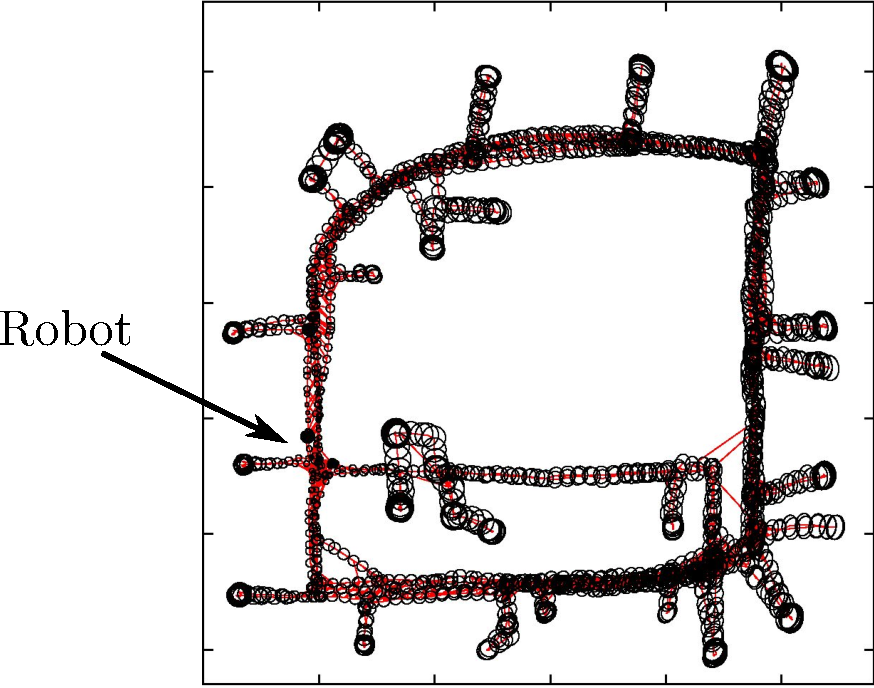
\includegraphics[width=0.2\textwidth]{pose_graph_relative_uncertainty.pdf}
    \end{figure}
    
\end{frame}

\begin{frame}
    \frametitle{Resumen de Pose-Graph}
    \note{Información extraída de https://youtu.be/uHbRKvD8TWg}
    
    \begin{itemize}
        \item El back-end del problema de SLAM puede ser resuelto aplicando Gauss-Newton
        \item La matriz $\linearSystemH$ es dispersa
        \item Que $\linearSystemH$ sea dispersa nos permite resolver el sistema lineal de manera eficiente
    \end{itemize}
    
\end{frame}

\begin{frame}
    \frametitle{Graph-Based SLAM con landmarks}
    \note{Información extraída de https://youtu.be/mZBdPgBtrCM}
    
   	\begin{figure}[!h]
        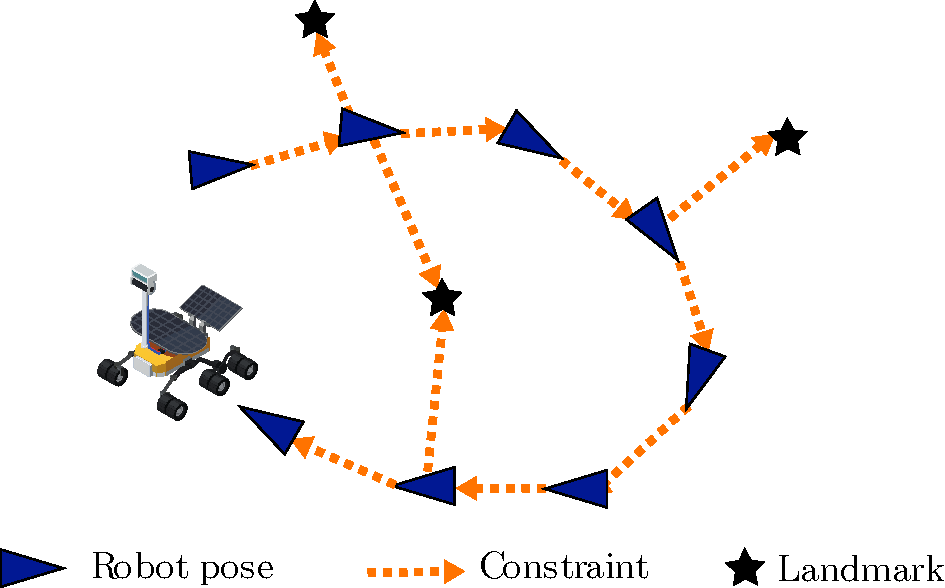
\includegraphics[width=0.6\textwidth]{images/pose_landmark_graph_example.pdf}
    \end{figure}
    
\end{frame}

\begin{frame}
    \frametitle{Observaciones de landmarks}
    \note{Información extraída de https://youtu.be/mZBdPgBtrCM}
    
    \begin{itemize}
		\item Observación esperada para un (x-y sensor\footnote{x-y sensor es un sensor cuyas mediciones tiene la forma (x,y), un punto de la escena. En un mundo 2D.})
   		\begin{figure}[!h]
			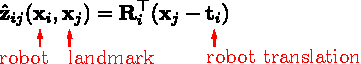
\includegraphics[width=0.6\textwidth]{images/pose_landmark_graph_expected_observation.pdf}
		\end{figure}
	\item Función error
	\begin{align*}
		\error_{ij}(\stateBold_{i}, \stateBold_{j}) &= \hat{\observationBold}_{ij} - \observationBold_{ij}\\
					&= \rotation_{i}^{\top}(\stateBold_{j}-\translation_{i}) - \observationBold_{ij}
	\end{align*}
    \end{itemize}
    
\end{frame}

\begin{frame}
    \frametitle{Bearing only obsevations (observaciones de ángulo)}
    \note{Información extraída de https://youtu.be/mZBdPgBtrCM}
    
    \begin{itemize}
		\item Un landmark es un punto 2D
		\item El robot observa el ángulo hacia el landmark
		\item Función de observación
   		\begin{figure}[!h]
			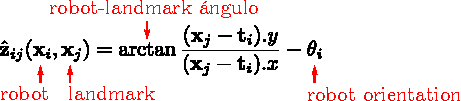
\includegraphics[width=0.6\textwidth]{images/pose_landmark_graph_bearing_observation.pdf}
		\end{figure}
		\item Función error
		\begin{equation*}
			\error_{ij}(\stateBold_{i},\stateBold_{j}) = \arctan{\dfrac{(\stateBold_{j}-\translation_{i}).y}{(\stateBold_{j}-\translation_{i}).x}} - \theta_{i} - \observationBold_{j}
		\end{equation*}
    \end{itemize}

    
\end{frame}

\begin{frame}
    \frametitle{Rango de la matriz H}
    \note{Información extraída de https://youtu.be/mZBdPgBtrCM}
    \begin{itemize}
		\item ¿Cuál es el rango de la matriz $\linearSystemH_{ij}$ para restricción pose-landmark 2D?
		\begin{itemize}
			\item El rango de $\linearSystemH_{ij}$ está determinado por el rando del Jacobiano $\jacobian_{ij}$ que a lo sumo es una matriz de $2 \times 5$. 2 porque la medición da información 2D y 5 por $\begin{bmatrix}	x & y & theta & l_{x} & l_{y} \end{bmatrix}$
			\item $\linearSystemH_{ij}$ no puede tener más que rango 2
			
				$rank(A^{\top} A) = rank(A^{\top}) = rank(A)$
		\end{itemize}
	
		\item ¿Cuál es el rango de la matriz $\linearSystemH_{ij}$ para restricción pose-landmark 2D?
		\begin{itemize}
			\item El rango de $\linearSystemH_{ij}$ está determinado por el rando del Jacobiano $\jacobian_{ij}$ que a lo sumo es una matriz de $1 \times 5$. 1 porque la medición da información 1D y 5 por $\begin{bmatrix}	x & y & theta & l_{x} & l_{y} \end{bmatrix}$
			\item $\linearSystemH_{ij}$ tiene rango 1
		\end{itemize}
		
    \end{itemize}
\end{frame}

\begin{frame}
    \frametitle{¿Dónde está el robot?}
    \note{Información extraída de https://youtu.be/mZBdPgBtrCM}
    \begin{itemize}
		\item El robot observa un landmark $(x,y)$
		\item ¿Dónde puede estar el robot relativo al landmark?
    \end{itemize}

	\only<1>{
	 	\begin{figure}[!h]
    	
\includegraphics[width=0.3\textwidth]{images/robot_pose_landmark_with_xy_sensor1.pdf}
    	\end{figure}
	}
 	
 	\only<2>{
 	\begin{figure}[!h]
		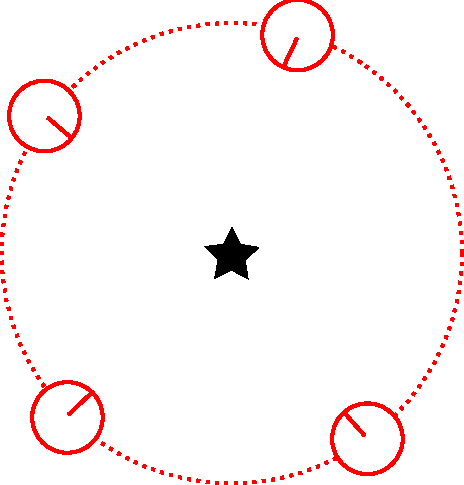
\includegraphics[width=0.3\textwidth]{images/robot_pose_landmark_with_xy_sensor2.pdf}
	\end{figure}
	El robot puede estar en cualquier lugar del círculo.\\
	Es un espacio de soluciones 1D (restringido por la distancia y la orientación del robot)
	}
\end{frame}

\begin{frame}
	\frametitle{¿Dónde está el robot?}
	\note{Información extraída de https://youtu.be/mZBdPgBtrCM}
	\begin{itemize}
		\item El robot observa un landmark (bearing-only)
		\item ¿Dónde puede estar el robot relativo al landmark?
	\end{itemize}
	
	\only<1>{
		\begin{figure}[!h]
			
\includegraphics[width=0.3\textwidth]{images/robot_pose_landmark_with_bearing_sensor1.pdf}
		\end{figure}
	}
	
	\only<2>{
		\begin{figure}[!h]
			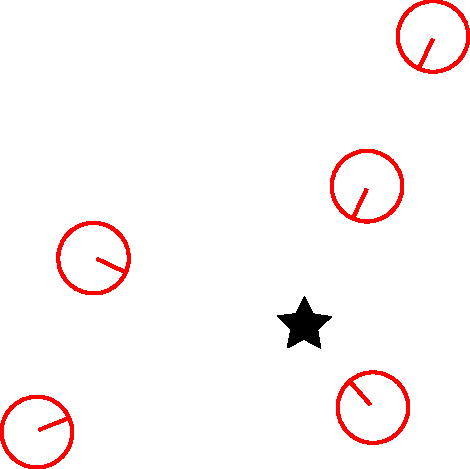
\includegraphics[width=0.3\textwidth]{images/robot_pose_landmark_with_bearing_sensor2.pdf}
		\end{figure}
		El robot puede estar en cualquier lugar lugar del plano xy. Siempre estará apuntando hacia el landmark.
		Es un espacio soluciones 2D (restringido por la orientación del robot).
	}
\end{frame}

\begin{frame}
    \frametitle{Rango}
    \note{Información extraída de https://youtu.be/mZBdPgBtrCM}
    \begin{itemize}
		\item En SLAM con landmark, el sistema puede quedar indeterminado
		\item El rango de $\linearSystemH$ es {\bf menor o igual} que la suma de los rangos de todas las observaciones
		\item Para determinar una {\bf solución única}, el sistema debe tener {\bf rango completo}
    \end{itemize}
	\only<2>{
		Preguntas:
		\begin{itemize}
			\item ¿Cuantas observaciones de landmarks 2D se necesitan para resolver la pose de un robot?
			\item ¿Cuantas observaciones bearing-only se necesitan para resolver la pose de un robot?
		\end{itemize}
	}
\end{frame}

\begin{frame}
    \frametitle{Sistema indeterminado}
    \note{Información extraída de https://youtu.be/mZBdPgBtrCM}
    \begin{itemize}
		\item No hay garantía que que un sistema tenga rango completo
		\begin{itemize}
			\item Los landmarks puede ser observados una sola vez
			\item El robot puede que no tenga información de odometría
		\end{itemize}
		\item Podemos lidiar con estos problemas utilizando un \emph{damping factor} para $\linearSystemH$
		\item En vez de resolver $\linearSystemH \vec{\Delta} \stateBold = - \linearSystemb$, resolvemos
		$(\linearSystemH + \lambda \vec{I}) \vec{\Delta} \stateBold = - \linearSystemb$
    \end{itemize}
\end{frame}

\begin{frame}
    \frametitle{Levenberg–Marquardt}
    \note{Información extraída de https://youtu.be/mZBdPgBtrCM}
    
    \footnotesize
    
    \begin{itemize}
		\item El damping factor $\lambda \vec{I}$ hace que el sistema sea definido positivo
		\item Es una suma ponderada del método de Gauss-Newton y el método de descenso por el gradiente
		\item El damping factor regula la convergencia usando acciones de backup/restore
    \end{itemize}

	\begin{algorithmic}[1]
		\Procedure{Levenberg–Marquardt}{$\stateBold$} \Comment{$\stateBold$: semilla inicial}
		\While (!converged)
		\State $\lambda =  \lambda_{\textrm{init}}$
		\State $<\linearSystemH, \linearSystemb> = buildLinearSystem(\stateBold)$
		\State $E = error(\stateBold)$
		\State $\stateBold_{\textrm{old}} = \stateBold$
		\State $\vec{\Delta}\stateBold = solveSparse((\linearSystemH + \lambda \vec{I}) \vec{\Delta} \stateBold = - \linearSystemb)$
		\State $\stateBold \mathrel{+}= \vec{\Delta}\stateBold$
		\If{$E < error(\stateBold)$}
		\State $\stateBold = \stateBold_{\textrm{old}}$
		\State $\lambda \mathrel{*}= 2$
		\Else
		\State $\lambda \mathrel{/}= 2$
		\EndIf
		\EndWhile
		\EndProcedure
	\end{algorithmic}

\end{frame}


\begin{frame}
    \frametitle{Bundle Adjustment}
    \note{Información extraída de https://youtu.be/BuRCJ2fegcc y de https://youtu.be/mZBdPgBtrCM}
    
    Bundle Adjustment es un caso
    
    \begin{itemize}
        \item Reconstrucción 3D basada en imágenes tomadas de diferentes puntos de vista
        \item Minimiza el error de reproyección en el plano de la imagen 2D
        \item No hay noción de odometría (pose-pose constraints)
        \item En general utiliza como método de minimización Levenberg-Marquart
        \item Desarrollado en el área de Fotogrametría\footnote{Fotogrametría es la técnica cuyo objeto es estudiar y definir con precisión la forma, dimensiones y posición en el espacio de un objeto cualquiera, utilizando esencialmente medidas hechas sobre una o varias fotografías de ese objeto} durante la década de 1950
    \end{itemize}
    
\end{frame}

\begin{frame}
	\frametitle{Bundle Adjustment}
	
	\begin{figure}
		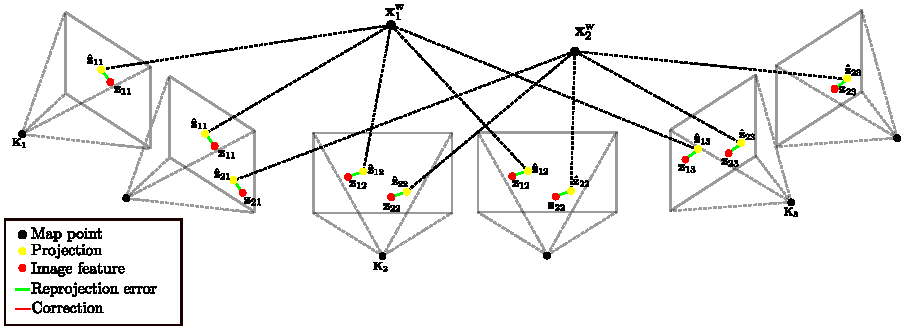
\includegraphics[width=\textwidth]{./images/ba_reprojection_error_before.pdf}
	\end{figure}
	
	\note{Ejemplo de ajuste de 3 keyframes que ven 2 puntos del mapa.\\
		k1 - x1 medición estéreo\\
		k1 - x2 medición derecha\\
		k2 - x1 medición estéreo\\
		k2 - x2 medición estéreo\\
		k3 - x1 medición izquierda\\
		k3 - x2 medición estéreo}
	
\end{frame}

\begin{frame}
	\frametitle{Bundle Adjustment}
	
	\begin{figure}
		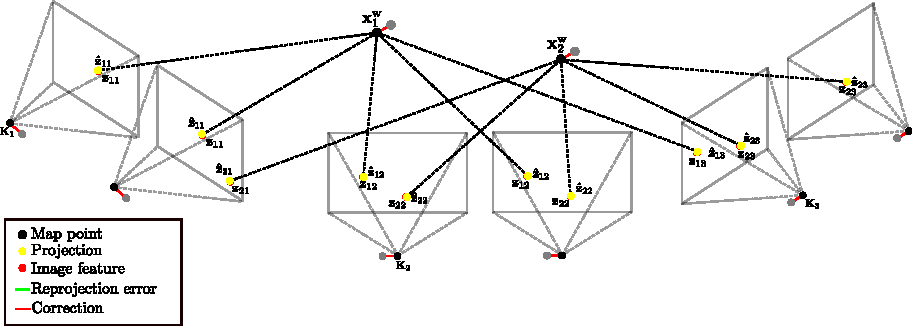
\includegraphics[width=\textwidth]{./images/ba_reprojection_error_after.pdf}
	\end{figure}
	
	\note{Ajustamos los keyframes y los puntos!!!\\
		Una ecuación de error por cada medición (6 en total).\\
		Nuevamente tenemos en cuenta la transformación rígida entre la cámara izquierda y la cámara derecha para las mediciones derechas.}
	
\end{frame}



